% manuscript_with_biblio.tex
% Autonomous variant of manuscript.tex. The APA bibliography contains only
% references cited in this manuscript and is embedded as a thebibliography
% environment; no external .bib file or BibTeX pass is required.

\documentclass{interact}

\usepackage[T1]{fontenc}
\usepackage[utf8]{inputenc}
\usepackage{epstopdf} 
\usepackage{graphicx}
\usepackage{booktabs}
\usepackage{array}
\usepackage{tabularx}
\usepackage{amsmath}
\usepackage{amssymb}
\usepackage{url}
\usepackage{xcolor}
\usepackage{mdframed}
\usepackage{setspace}

% Slightly more open line spacing for readability
\setstretch{1.25}

% Light gray callout for NLG quotes: box matches default quote width
\definecolor{quoteboxbg}{gray}{0.94}
\mdfdefinestyle{quotebox}{%
  backgroundcolor=quoteboxbg,
  hidealllines=true,
  leftmargin=\leftmargin,
  rightmargin=\leftmargin,
  innertopmargin=10pt,
  innerbottommargin=10pt,
  innerleftmargin=10pt,
  innerrightmargin=10pt,
  skipabove=\topsep,
  skipbelow=\topsep,
}
\renewenvironment{quote}{%
  \begin{mdframed}[style=quotebox]%
}{%
  \end{mdframed}%
}

% Float placement: prefer top of page, keep floats near their callouts,
% and flush deferred floats before major section breaks when needed.
\usepackage{flafter}
\usepackage{placeins}
\renewcommand{\topfraction}{0.95}
\renewcommand{\bottomfraction}{0.8}
\renewcommand{\textfraction}{0.05}
\renewcommand{\floatpagefraction}{0.8}
\setcounter{topnumber}{3}
\setcounter{bottomnumber}{2}
\setcounter{totalnumber}{4}
\setlength{\floatsep}{4pt plus 1pt minus 1pt}
\setlength{\textfloatsep}{8pt plus 2pt minus 2pt}
\setlength{\intextsep}{8pt plus 2pt minus 2pt}
\raggedbottom

% APA author-year (Taylor & Francis Interact + APA)
\usepackage[natbibapa,nodoi]{apacite}
\setlength\bibhang{12pt}
\renewcommand\bibliographytypesize{\fontsize{10}{12}\selectfont}

\usepackage{hyperref}

\begin{document}

\articletype{Software Tool Article}

\title{CADEMAS-ML: A Software Tool for Context-Aware Cooperative and Explainable Automated Decision-Making}

\author{
\name{Pavel Novoa-Hern\'{a}ndez\textsuperscript{a}\thanks{CONTACT Pavel Novoa-Hern\'{a}ndez. Email: pnovoahe@ull.edu.es} and David A. Pelta\textsuperscript{b}}
\affil{\textsuperscript{a}Dept. Computer Engineering and Systems, Universidad de La Laguna, San Crist\'{o}bal de La Laguna, Spain; \textsuperscript{b}Dept. Computer Science and Artificial Intelligence, Universidad de Granada, Granada, Spain}
}

\maketitle

\begin{abstract}
Automated decision-making outputs are often interpreted without the organizational context in which action is taken. This paper presents CADEMAS-ML, an open-source software tool that operationalizes the Cooperative Automated Decision-Making Systems (CADEMAS) framework for context-aware case prioritization. Multiple predictive models act as cooperating decision units; their outputs are aggregated into a risk score and combined with contextual alignment encoded as configurable fuzzy rules. The tool explains individual recommendations by decomposing the priority score, attributing local predictive drivers, and tracing fuzzy-rule memberships, and it evaluates ranking robustness under alternative balances between prediction and context. A reproducible employee-attrition example with four departmental models and a digital-transformation policy demonstrates how predictive risk and contextual alignment play distinct roles in prioritization and how users can inspect inputs, intermediate scores, final rankings, and explanations before acting. The article describes the implementation, operation, demonstration setup, and resulting module outputs. Source code, an example bundle, and documentation are available under an MIT license.
\end{abstract}

\begin{keywords}
automated decision-making systems; fuzzy decision making; context-aware decision support; machine learning; prioritization; cooperative systems
\end{keywords}

\section{Introduction}\label{sec:intro}

Automated decision-making (ADM) systems have become an integral part of modern organizations. Following the broad understanding of ADM as computational processes that produce ratings, recommendations, decisions, predictions, or related outputs from data and predefined objectives \citep{EIP2022}, such systems may include machine-learning classifiers, rule-based procedures, optimization models, simulation components, or other algorithmic decision units. In practice, predictive and classification models are among the most common instantiations, supporting tasks such as credit scoring, fraud detection, medical triage, customer churn analysis, and human resources management.

Despite these advances, an important limitation remains. The outputs generated by ADM units, such as recommendations, ratings, class probabilities, or risk scores, are often interpreted in isolation from the organizational environment in which decisions are ultimately made \citep{Tariq2024a,Deliu2026}. In practice, a technically plausible automated output rarely provides sufficient guidance for action. The appropriate response depends on contextual factors such as organizational priorities, resource constraints, departmental objectives, regulatory constraints, and prevailing strategic conditions. As a result, identical automated assessments may lead to different decisions under different circumstances.

This observation highlights the cooperative nature of real-world decision-making \citep{Borkotokey2019,Tariq2024a}. Decisions are seldom based on a single decision agent or automated component. Organizations frequently rely on heterogeneous units developed for different departments, objectives, data sources, or stakeholder groups. Their outputs must therefore be harmonized into a coherent assessment before they can support action. At the same time, domain experts contribute contextual knowledge that cannot always be represented through precise numerical rules. Such knowledge is often expressed through gradual concepts and linguistic assessments that reflect uncertainty, preference, and strategic intent.

Fuzzy logic provides a well-established mathematical framework for representing this type of contextual reasoning \citep{PerezCanedo2023,Lamata2020}. Through fuzzy sets and linguistic variables, experts can model concepts such as urgency, strategic relevance, or suitability in a transparent and interpretable manner. This makes fuzzy approaches particularly attractive for decision-support environments in which quantitative predictions must be complemented by qualitative contextual considerations.

To address these challenges, \citet{NovoaHernandez2026} proposed \textit{CADEMAS} (Cooperative Automated Decision-Making Systems), a conceptual framework for coordinating heterogeneous automated decision units. The framework separates the generation of decision evidence from its contextual evaluation, allowing outputs from multiple decision units to be integrated and subsequently assessed according to scenario-specific conditions and priorities.

The practical value of this approach was subsequently demonstrated by \citet{Godz2026}, who instantiated CADEMAS in the context of employee-attrition prevention. In that work, predictive machine-learning models developed from different organizational perspectives were treated as cooperating decision units and combined with contextual organizational policies to support case prioritization. The results showed that the framework could effectively integrate predictive evidence and contextual knowledge within a coherent decision-making process.

Although CADEMAS provides a solid conceptual foundation for cooperative and context-aware decision-making, its practical application typically involves a non-trivial implementation effort. In particular, users must define how case data are distributed across multiple decision units, how their outputs are collected and aligned, how these outputs are integrated, and how the resulting decision proposal is evaluated under explicit contextual assumptions. While these steps are conceptually well-defined, they must be specified and coordinated for each new domain or dataset, creating operational overhead for both researchers and decision-makers.

Beyond this implementation effort, decision-support settings also require additional capabilities that are often critical in practice, such as assessing the robustness of decisions under alternative policy configurations and providing clear, auditable explanations of how individual recommendations are derived \citep{Arrieta2020}. Influential approaches to case-level explanation, including Shapley-value methods such as SHAP \citep{Lundberg2017,Li2024}, illustrate why local attribution has become central to trustworthy decision support. These requirements are particularly relevant in organizational environments where decisions must be justified, audited, and analyzed under changing contextual conditions. However, they are not explicitly addressed in the original CADEMAS formulation nor in subsequent application-focused instantiations.

This paper addresses these requirements by presenting \textbf{CADEMAS-ML}, a software tool that operationalizes the CADEMAS framework for cooperative and context-aware automated decision-making. The contribution is a reusable, auditable implementation---not a new attrition predictor. The main contributions of this work are as follows:
\begin{itemize}
\item The development of CADEMAS-ML, an open-source software tool that implements the CADEMAS framework for context-aware cooperative decision-making using machine-learning models as automated decision units.
\item The integration of predictive analytics, fuzzy contextual reasoning, and explainable decision support within a unified prioritization process, enabling transparent justification and case-level interpretability through local model-agnostic attribution.
\item A robustness-analysis module that allows decision-makers to assess the sensitivity and stability of prioritization outcomes under alternative contextual policies and preference configurations.
\item A reproducible software demonstration in an employee-attrition prevention scenario involving multiple predictive models and an explicit organizational context.
\end{itemize}

The explainability and robustness capabilities introduced in this work are central to its operational contribution. They complement the original CADEMAS formulation, which is primarily architectural, as well as prior application-oriented instantiations, by supporting an interactive decision-support workflow in which users can inspect the rationale behind individual prioritizations and assess their stability under alternative contextual assumptions. This shifts the focus from producing a single prioritization outcome to enabling its interpretation, justification, and analysis in practice.

The remainder of the paper is organized as follows. Section~\ref{sec:background} reviews the CADEMAS framework and related decision-support work. Section~\ref{sec:methods} describes the implementation, operation, and employee-attrition demonstration setup. Section~\ref{sec:results} presents the outputs exposed by the user-facing modules. Section~\ref{sec:discussion} discusses the practical and research implications of the software, its limitations, and directions for further development.

\section{Background and related works}\label{sec:background}

This section sets out the conceptual foundations on which CADEMAS-ML builds. We first revisit the CADEMAS framework and formalize it for the prioritization setting addressed here (Section~\ref{sec:cademas}). We then situate the tool among related cooperative-decision frameworks and application-oriented decision-support systems, clarifying the gap it is designed to fill (Section~\ref{sec:related}).

\subsection{CADEMAS framework}\label{sec:cademas}

As introduced in Section~\ref{sec:intro}, CADEMAS \citep{NovoaHernandez2026} provides a general structure for designing systems in which multiple automated decision-making units cooperate to produce contextually aligned decisions. As noted there, its motivation is not limited to prediction: organizational decisions rarely emerge from a single autonomous unit with a single representation of the problem, and may instead depend on heterogeneous signals produced by classifiers, optimization models, simulation components, rule-based systems, large-language-model agents, or institutional procedures, each with its own assumptions, data access, output type, and reliability level.

To formalize this idea for the prioritization setting addressed in this paper, let $\mathcal{X} = \{x_1, \dots, x_n\}$ denote the case dataset, and let $\mathcal{A} = \{A_1, \dots, A_K\}$ represent a collection of ADM units. In the general CADEMAS framework, each $A_k$ may produce an output $o_k(x_i)$ whose semantics are not necessarily probabilistic: it may be a class, a score, a ranking, a symbolic recommendation, a rule activation, or another decision object. A decision-integration layer is therefore responsible for transforming these heterogeneous outputs into a shared representation and synthesizing them into an integrated proposal.

CADEMAS-ML implements the specialization in which the ADM units are predictive models $\mathcal{M}=\{M_1,\ldots,M_K\}$ and the harmonized output of model $M_k$ for case $x_i$ is a positive-class probability $\hat{p}_{ik}\in[0,1]$. Since the models may differ in performance and trustworthiness, each $M_k$ is assigned a confidence weight $w_k\geq0$, with $\sum_{k=1}^{K}w_k=1$. The weights can be derived from validation metrics, expert judgment, or governance constraints. Using the notation retained throughout the rest of the article, the integrated predictive risk is
\begin{equation}
R_i = \sum_{k=1}^{K} w_k \hat{p}_{ik}.
\end{equation}

Rather than treating the integrated output as the final decision criterion, CADEMAS introduces an explicit contextual layer that captures organizational priorities, policies, constraints, and scenario-dependent considerations. The original framework does not prescribe a single context formalism. Context may be represented through crisp rules, utility functions, regulatory constraints, fuzzy propositions, or other evaluative mechanisms. CADEMAS-ML follows the attrition application of \citet{Godz2026} and uses fuzzy logic because it supports gradual degrees of satisfaction instead of binary rules. Let $\mathcal{Q}=\{r_1,\ldots,r_L\}$ denote the contextual rules and let $\mu_r(x_i)\in[0,1]$ be the degree to which case $x_i$ satisfies rule $r$. These values are aggregated into the context-alignment score
\begin{equation}
C_i = H\big(\mu_{r_1}(x_i), \dots, \mu_{r_L}(x_i)\big),
\end{equation}
where $H: [0,1]^L \rightarrow [0,1]$ is an aggregation operator that can take different forms depending on the decision policy (e.g., t-norms, averages, or hierarchical compositions).

The final prioritization score combines predictive risk and context alignment:
\begin{equation}
P_i(\lambda)=\lambda R_i+(1-\lambda)C_i,\qquad \lambda\in[0,1].
\end{equation}
The balance parameter $\lambda$ makes the trade-off explicit. A key design principle inherited from CADEMAS is the separation between the integrated ADM proposal and its contextual interpretation. In this specialization, $R_i$, $C_i$, and $P_i(\lambda)$ distinguish what the predictive models suggest, what the organization considers relevant, and how both sources are combined.

The framework was instantiated in employee-attrition prevention by \citet{Godz2026}. In that application, multiple machine-learning models were trained on different organizational perspectives, including Human Resources, Finance, Operations and Development, and a wellbeing-oriented perspective identified as Culture and Wellbeing in the software bundle. Each model acts as an ADM unit, and their outputs are combined using weights derived from validation performance, specifically AUC. In parallel, the contextual layer encodes scenario-dependent organizational priorities (e.g., economic crisis or digital transformation settings) using fuzzy membership functions and rule-based structures.

Although this instantiation demonstrates the practicality of the framework, it represents only one possible configuration. In general, CADEMAS is designed to remain flexible across several dimensions, including the type of automated decision units, the semantics of their outputs, the mechanism used for aligning heterogeneous decision signals, the integration strategy, and the way contextual information is incorporated into the final decision.

CADEMAS-ML implements specific design choices for these components to provide a concrete and reproducible software realization of the framework. Within the general CADEMAS formulation, however, these elements remain configurable: confidence weights can be derived from different performance criteria, aggregation strategies may reflect alternative decision policies, and the final prioritization can be adjusted to capture different trade-offs between predictive evidence and contextual constraints.

This configurability is essential for adapting CADEMAS to heterogeneous organizational environments and motivates the need for a software layer that operationalizes these design decisions in a systematic and reusable manner.

\subsection{Related frameworks and decision-support applications}\label{sec:related}

Recent research has increasingly recognized that effective decision support requires more than accurate isolated models. In many application domains, decisions emerge from the interaction between automated units, expert knowledge, and contextual considerations that may change over time. For clarity, it is useful to distinguish two related but different bodies of work: general cooperative-decision frameworks, which address how multiple decision entities interact, and application-oriented decision-support systems, which implement concrete methods for a domain or family of decision problems.

At the framework level, cooperative game theory offers one formal perspective on how decision-making entities with heterogeneous roles or attributes may combine their contributions, including settings in which each agent is characterized by multiple attributes rather than a single payoff value \citep{Borkotokey2019}. CADEMAS does not adopt this game-theoretic formulation, but shares its concern with making cooperation among heterogeneous entities explicit. At the operational level, \citet{Tariq2024a} propose an AI-to-collaborator (A2C) framework in which humans and AI systems share decision authority through explicit interaction mechanisms. Related work on hybrid intelligence emphasizes that authority distribution and human interpretive capacity should be modeled separately, because the level of AI integration and the cognitive flexibility of human decision-makers jointly shape decision quality and accountability \citep{Deliu2026}. A neighboring line of work examines cooperation among multiple AI agents, including LLM-based multi-agent reinforcement learning \citep{Sun2024}. These contributions provide relevant points of comparison because they address cooperation among decision entities. However, their main focus is not the reusable implementation of a CADEMAS-like workflow in which heterogeneous ADM outputs are explicitly separated from context modulation and final prioritization.

A related theoretical thread connects cooperative game theory to case-level explanation. The Shapley value distributes a joint outcome among players according to their averaged marginal contributions \citep{Borkotokey2019} and has been adopted in explainable artificial intelligence as a principled attribution mechanism. SHapley Additive exPlanations (SHAP) \citep{Lundberg2017} treat model features as players and decompose each prediction into additive feature contributions with axiomatic guarantees; recent surveys document the breadth of this cooperative-to-XAI bridge \citep{Li2024}. This literature motivates the inclusion of an explicit explanation module in CADEMAS-ML. The current implementation does not compute Shapley values over features: because the uploaded H2O MOJO models are treated as black boxes and may include stacked ensembles, the tool uses a model-agnostic perturbation procedure instead. The purpose is nonetheless the same as in Shapley-inspired XAI: to make the local drivers of a recommendation inspectable alongside the cooperative and contextual scores.

At the application and decision-support level, substantial progress has been made in fuzzy decision support, multi-criteria decision making, and hybrid fuzzy-ML workflows. Applications such as \textsc{MakeDecision} \citep{Wieckowski2024} and the fuzzy DEMATEL-based tool of \citet{Chekry2024} emphasize transparency and traceability by exposing intermediate calculations to users. A related stream has explored hybrid pipelines that combine expert judgment, causal weighting, and predictive components in domain-specific settings \citep{Abdulgader2018,Sahraei2022,Ozkurt2025}. Recent work has also extended the fuzzy toolbox through aggregation operators that account for interactions among decision attributes, capturing dependency structures that simple weighted averages cannot represent \citep{Kacprzyk2022}. The importance of explainability in AI-based decision support has been broadly recognized: any automated system whose outputs must be justified or audited requires transparent mechanisms to convey its reasoning to stakeholders \citep{Arrieta2020}, a requirement increasingly addressed through XAI techniques, including Shapley-value attribution \citep{Lundberg2017,Li2024}, in hybrid ranking and prediction pipelines \citep{Ozkurt2025}. These contributions demonstrate the value of combining data-driven evidence with contextual or expert-defined criteria, but most are tailored to particular methods or domains rather than organized around the CADEMAS decomposition of ADM units, integration, context, and final prioritization.

Open-source fuzzy and MCDM libraries, including \textsc{pyFDM} \citep{Wieckowski2022}, \textsc{PyIFDM} \citep{Wieckowski2023}, the \textsc{IFMCDM} package of \citet{Roszkowska2024}, the \textsc{Eligere} platform \citep{Grazioso2023}, and the intuitionistic fuzzy dimensional-analysis approach of \citet{PerezDominguez2024}, are also relevant. They improve reproducibility and provide reusable computational building blocks.

\begin{table}[!tb]
\tbl{Comparison of representative application-oriented decision-support works related to CADEMAS-ML.}
{\footnotesize
\begin{tabularx}{\textwidth}{>{\raggedright\arraybackslash}p{1.85cm} >{\raggedright\arraybackslash}X >{\centering\arraybackslash}p{1.35cm} >{\centering\arraybackslash}p{1.35cm} >{\centering\arraybackslash}p{1.35cm} >{\raggedright\arraybackslash}X}
		\toprule
		\textbf{Work} & \textbf{Decision-support focus} & \textbf{Multiple ADM units} & \textbf{Explicit context layer} & \textbf{Case-level XAI} & \textbf{Relation to CADEMAS-ML} \\
		\midrule
		\citet{Godz2026} & Employee-attrition prevention using CADEMAS with departmental ML models & Yes & Yes & No & Direct application that motivates the implemented workflow \\
		\citet{Tariq2024a} & Human--AI collaborative decision framework with automated, augmented, and collaborative modes & Partly & Partly & No & Strong framework-level precedent, but not a configurable fuzzy/ML prioritization workflow \\
		\citet{Wieckowski2024} & Auditable fuzzy MCDM through a web-based tool & No & Partly & No & Strong transparency, but no cooperative ADM integration layer \\
		\citet{Chekry2024} & Open-source fuzzy DEMATEL decision-support tool & No & Partly & No & Traceable fuzzy causal analysis, but method-specific rather than CADEMAS-like \\
		\citet{Ozkurt2025} & Hybrid fuzzy MCDM, ML, and XAI for transparent ranking and prediction & Partly & Partly & Partly & Combines ranking, prediction, and XAI, but lacks a general cooperative ADM architecture \\
		\citet{Sahraei2022} & Fuzzy DEMATEL/BWM/ANP pipeline for spatial risk prioritization & No & Partly & No & Explicit causal weighting under uncertainty, but application-specific \\
		\midrule
		CADEMAS-ML (this work) & Configurable prioritization with ML-based ADM units, fuzzy context scenarios, and local case explanation & Yes & Yes & Yes & Operationalizes CADEMAS for reusable, explainable ML-driven decision support \\
		\bottomrule
	\end{tabularx}}
\label{tab:related}
\end{table}

Table~\ref{tab:related} summarizes representative application-oriented contributions in these areas. Three observations emerge from this comparison. First, published systems already provide strong ingredients for transparent decision support, including human--AI collaboration, auditable fuzzy MCDM, hybrid ranking pipelines, and reusable software libraries \citep{Tariq2024a,Wieckowski2024,Ozkurt2025,Wieckowski2022}. Second, these ingredients are usually developed in isolation. Third, few systems combine cooperative multi-ADM integration, an explicit fuzzy context layer, and case-level explanation in one reusable workflow. What remains missing is an operational implementation that keeps these capabilities configurable and auditable together.

CADEMAS-ML is designed to address this gap for the predictive-model setting. Building on the framework and its attrition instantiation discussed above, it provides a configurable software implementation in which ML-based ADM outputs, contextual reasoning, and case-level explanation coexist as explicit and auditable components of the decision-making process. The source code is publicly available under an MIT license (Section~\ref{sec:software}); the main contribution is the operationalization of the CADEMAS decomposition in a reusable decision-support tool.

\section{Methods}\label{sec:methods}

This section presents CADEMAS-ML as a software realization of one concrete CADEMAS specialization: cooperative prioritization supported by multiple predictive ADM units and an explicit fuzzy context layer. We first describe the implementation (architecture, scoring, explanation, and robustness) and then explain how the tool is operated. The final subsection defines the employee-attrition demonstration used to report the software outputs in Section~\ref{sec:results}.

\subsection{Implementation}\label{sec:implementation}

CADEMAS-ML \citep{cademasml2026} is not a domain-specific attrition script. It is an operational implementation of CADEMAS for the case in which the cooperating ADM units are predictive models. In line with \citet{NovoaHernandez2026}, the software keeps partial automated assessments separate from their contextual interpretation. Its contribution is to make this separation executable for ML-based decision support. Predictive components, contextual rules, and decision policies are configured explicitly and can be inspected through the interface. Thus, the attrition study of \citet{Godz2026} becomes one possible configuration of the tool, not its only intended use.

\begin{figure}[!tb]
\centering
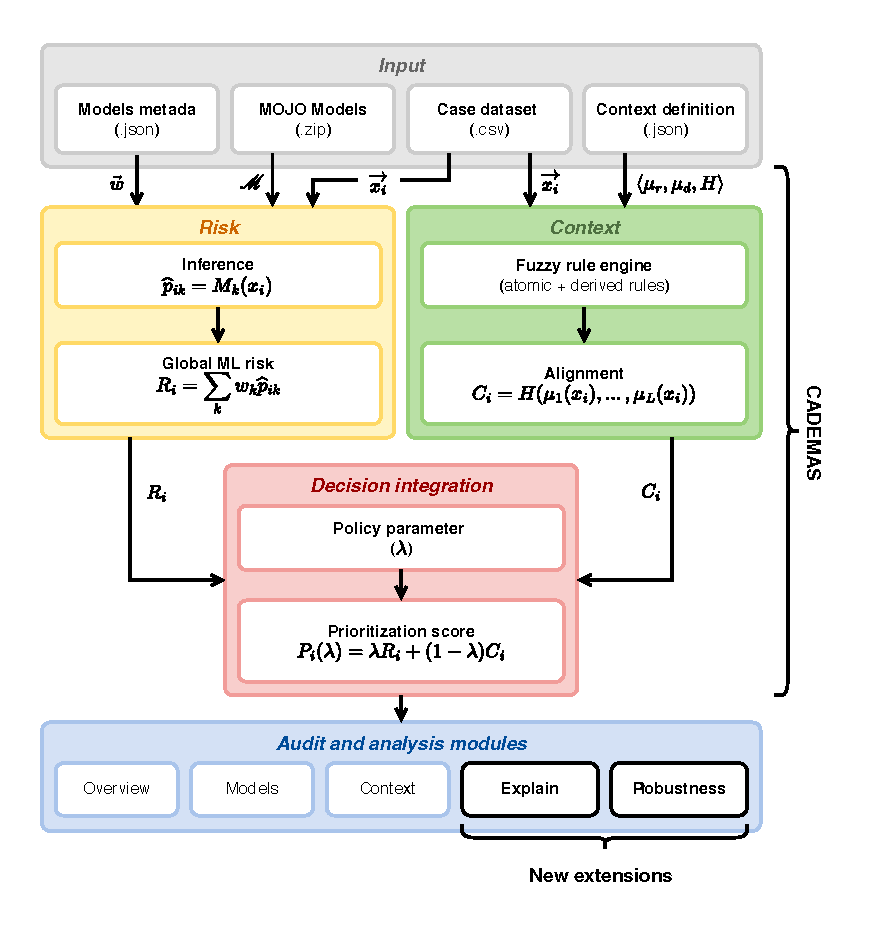
\includegraphics[width=\textwidth]{figures/architecture.pdf}
\caption{Operational architecture of the CADEMAS-ML application. The software instantiates the CADEMAS \citep{NovoaHernandez2026} architecture as a configurable vertical pipeline in which predictive risk and contextual alignment are computed independently before being integrated into a prioritization score.}
\label{fig:cademas_arch}
\end{figure}

The application is implemented in Python and combines a Streamlit \citep{streamlit} front end, H2O \citep{H2O.ai2026} inference, and a vectorized fuzzy-context engine. The six user-facing modules are \textit{Home} for configuration, \textit{Overview} for integrated prioritization, \textit{Models} for predictive outputs, \textit{Context} for fuzzy-policy auditing, \textit{Explain} for case-level interpretation, and \textit{Robustness} for sensitivity analysis. Interactive visual analytics are rendered with Altair \citep{VanderPlas2018}.

A run starts from four inputs: the case dataset, the MOJO models, a model-metadata JSON file, and one or more context JSON files. These inputs map naturally onto the CADEMAS layers. The dataset and configuration files act as the input manager. The MOJO files instantiate the ADM units in this ML specialization. Their weighted probabilistic outputs form the integrated predictive risk. The fuzzy-rule engine provides the contextual model. The final layer combines both streams through a user-adjustable policy parameter. Figure~\ref{fig:cademas_arch} summarizes this architecture.

\subsubsection{Cooperative predictive risk}

The predictive layer follows the cooperative aggregation principle of CADEMAS as specialized in the attrition instantiation of \citet{Godz2026}. CADEMAS-ML exposes that specialization as a reusable software component. Let $\mathcal{X}=\{x_1,\ldots,x_n\}$ be the case dataset and let $\mathcal{M}=\{M_1,\ldots,M_K\}$ be the uploaded predictive ADM units. Each model $M_k$ produces, for case $x_i$, a positive-class probability
\[
\hat{p}_{ik} \in [0,1].
\]
The models need not use the same feature subset. Each MOJO receives the available case matrix and uses its internal schema to select the required variables. The contribution of each component is controlled by a non-negative confidence weight $w_k$. This weight is computed from a user-selected validation metric $s_k$:
\begin{equation}
w_k = \frac{s_k}{\sum_{\ell=1}^{K} s_\ell}, \qquad \sum_{k=1}^{K}w_k=1.
\label{eq:model_weights}
\end{equation}
The cooperative predictive-risk score is then
\begin{equation}
R_i=\sum_{k=1}^{K}w_k\hat{p}_{ik}.
\label{eq:ml_risk}
\end{equation}
This mathematical form is the ML-specific realization of the more general CADEMAS decision-integration layer. The improvement introduced by CADEMAS-ML is practical configurability. Users can upload any number of compatible MOJO models, read model metadata from JSON, and choose the validation metric used for weighting.

\subsubsection{Configurable fuzzy context model}

The context layer is where CADEMAS-ML most clearly turns the conceptual framework into an operational artifact. The role of context follows \citet{NovoaHernandez2026}, and the use of fuzzy propositions follows the attrition application in \citet{Godz2026}. The difference is that CADEMAS-ML does not hard-code those contexts. It represents them as JSON specifications. The same formalism can therefore be reused with other domains, rule families, and decision policies.

Formally, a context is defined as a collection of fuzzy propositions. Let $V_r$ be a case attribute and let $\tilde{F}_r$ be a fuzzy set representing a linguistic predicate over the universe of $V_r$. For case $x_i$, an atomic rule $r$ evaluates the proposition ``$V_r$ is $\tilde{F}_r$'' as
\begin{equation}
\mu_r(x_i)=\mu_{\tilde{F}_r}(x_{ir}) \in [0,1],
\label{eq:atomic_mu}
\end{equation}
where $x_{ir}$ denotes the value of attribute $V_r$ for case $x_i$. The implementation supports triangular, trapezoidal, linear increasing, and linear decreasing membership functions. It also supports categorical maps and categorical sets. The former assign degrees directly to symbolic values. The latter group categories into linguistic labels that can be scored later in derived rules.

Atomic rules may include activation conditions. If $m_r(x_i)\in\{0,1\}$ denotes whether the \texttt{when} condition of rule $r$ is satisfied for case $x_i$, the effective membership is
\begin{equation}
\mu_r^{*}(x_i)=m_r(x_i)\mu_r(x_i),
\label{eq:conditional_mu}
\end{equation}
with $m_r(x_i)=1$ for unconditional rules. This makes it possible to represent policies such as department-specific salary suitability without duplicating datasets or writing procedural code.

Beyond atomic rules, CADEMAS-ML allows the definition of derived rules. A derived rule $d$ combines a subset of already computed memberships through an aggregation operator $G_d$:
\begin{equation}
\mu_d(x_i)=G_d\left(\mu_{r_1}^{*}(x_i),\ldots,\mu_{r_q}^{*}(x_i)\right).
\label{eq:derived_mu}
\end{equation}
The implemented operators are minimum-based \texttt{AND}, maximum-based \texttt{OR}, algebraic \texttt{PRODUCT}, and arithmetic \texttt{AVERAGE}. The context-alignment score is then obtained by applying a final aggregation policy $H$ to selected atomic and derived memberships:
\begin{equation}
C_i = H\left(\mu_1(x_i),\ldots,\mu_L(x_i)\right).
\label{eq:context_score}
\end{equation}
The function $H$ can be selected interactively or specified as a declarative logic tree in the context JSON. This captures the attrition instantiation in \citet{Godz2026}, but makes it portable. It also lets organizations express conservative, compensatory, hierarchical, or conditional contextual policies without changing the application code. The closed-form specification of the context used in the example is reported in Appendix~\ref{app:context_specs}.

All atomic and derived memberships are retained as an audit matrix. The final context score is therefore not a black-box modifier of the ML risk. It can be decomposed into the rule activations that produced it.

\subsubsection{Decision integration and robustness}

Predictive risk and contextual alignment remain separate until the final decision stage. For a fixed policy parameter $\lambda\in[0,1]$, CADEMAS-ML computes the prioritization score as
\begin{equation}
P_i(\lambda)=\lambda R_i+(1-\lambda)C_i.
\label{eq:priority_lambda}
\end{equation}
The interpretation is direct. A value $\lambda=1$ produces a risk-driven ranking. A value $\lambda=0$ produces a context-driven ranking. Intermediate values encode explicit trade-offs between both components.

The robustness module is a specific improvement of CADEMAS-ML over the previous static attrition instantiation. Let $\Lambda=\{\lambda_0,\ldots,\lambda_q\}$ be a finite grid of policy values. For each $\lambda\in\Lambda$, the tool computes the score vector $P(\lambda)$ and the ranking
\begin{equation}
r_i(\lambda)=1+\left|\{j: P_j(\lambda)>P_i(\lambda)\}\right|,
\label{eq:rank_lambda}
\end{equation}
with deterministic tie-breaking by case order. This produces a rank trajectory for every case. CADEMAS-ML summarizes these trajectories through three complementary Altair views: a bump chart, a ranks box plot, and a rank-acceptability heatmap. The bump chart shows how each case moves as $\lambda$ changes. The box plot summarizes the distribution of ranks over $\Lambda$; cases are ordered by median rank and interquartile range. Finally, the rank acceptability index estimates how often a case attains a given rank:
\begin{equation}
b_i^r = \frac{1}{|\Lambda|}\sum_{\lambda\in\Lambda}\mathbf{1}\{r_i(\lambda)=r\}.
\label{eq:rank_acceptability}
\end{equation}
Together, these indicators distinguish stable priorities from policy-sensitive cases.

\subsubsection{Case-level explanation and natural-language recommendations}

A second improvement introduced by CADEMAS-ML is the \textit{Explain} module. The original CADEMAS framework specifies the separation between ADM outputs, context evaluation, and final decision integration, but it does not prescribe a case-level explanation mechanism. Similarly, the attrition instantiation of \citet{Godz2026} reports contextual prioritization outcomes, but does not provide an interactive module that explains individual cases in natural language. CADEMAS-ML fills this gap by storing intermediate artifacts during the analysis run and exposing them through a four-part local explanation.

For a selected case $x_i$, the first explanation level decomposes the final score in Equation~\eqref{eq:priority_lambda} into its two additive components:
\begin{equation}
P_i(\lambda)=\underbrace{\lambda R_i}_{\text{predictive contribution}}+
\underbrace{(1-\lambda)C_i}_{\text{contextual contribution}}.
\label{eq:priority_decomposition}
\end{equation}
This decomposition makes explicit whether the prioritization is mainly driven by predictive risk, contextual alignment, or a balance between both.

The second level provides local ML attribution. Since the uploaded H2O AutoML MOJO models are treated as black-box predictive ADM units and may include stacked ensembles, CADEMAS-ML uses a model-agnostic perturbation procedure rather than relying on model-specific SHAP values. For each model $M_k$ and feature $f$, the tool compares the original predicted probability with the prediction obtained after replacing the value of $f$ by a cohort baseline $b_f$ (median for numerical variables and mode for categorical variables):
\begin{equation}
\Delta_{ikf}=\hat{p}_{ik}(x_i)-\hat{p}_{ik}(x_i^{(f \leftarrow b_f)}).
\label{eq:local_attribution_model}
\end{equation}
The model-specific effects are aggregated with the same confidence weights used for the cooperative predictive risk:
\begin{equation}
\Delta_{if}=\sum_{k=1}^{K} w_k \Delta_{ikf}.
\label{eq:local_attribution_global}
\end{equation}
Positive values indicate features whose observed value increases the local predicted risk relative to the cohort baseline, while negative values indicate features whose observed value decreases it. These quantities are expressed in probability points and should be interpreted as approximate local effects, not as causal impacts.

The third level traces the contextual component by presenting the fuzzy memberships $\mu_r(x_i)$ of the atomic and derived rules that produced $C_i$. This connects the numerical context score with the policy rules encoded in the JSON context specification. Finally, the fourth level generates a deterministic natural-language summary. The text combines the priority score, the balance parameter $\lambda$, the risk and context levels, the most relevant ML drivers, the most relevant contextual drivers or bottlenecks, and a generic tier-based recommendation. The recommendation uses $P_i(\lambda)$: \textit{Tier 1} for high priority, \textit{Tier 2} for medium or borderline priority requiring manual qualitative review, and \textit{Tier 3} for low priority under the current prediction and context guidelines.

\subsection{Operation}\label{sec:operation}

CADEMAS-ML is distributed as an open-source Python application \citep{cademasml2026}. Local execution requires Python~3.11 and Java~17 or later; the Java runtime is required by H2O MOJO loading. After the Python dependencies listed in the repository are installed, the interface is launched with Streamlit from the application entry point \texttt{app/app\_v1.py}. The repository README documents these steps.

A typical analysis has four stages. First, the user supplies or loads the four inputs required by the architecture: a case dataset, H2O MOJO models, a model-metadata JSON file, and one or more context JSON files. Second, the user selects the validation metric used for model weighting, chooses a context specification, and sets the balance parameter $\lambda$. Third, \textit{Run analysis} executes MOJO inference, fuzzy context evaluation, and score integration. Fourth, the resulting artifacts are inspected in the \textit{Overview}, \textit{Models}, \textit{Context}, \textit{Explain}, and \textit{Robustness} modules. No additional compilation of the predictive models is required at run time: the uploaded MOJO archives are consumed as they are. Appendix~\ref{app:input_summary} summarizes the input contract, while Supplementary Material~S1 provides the complete field-level specification and minimal examples.

\subsection{Employee-attrition demonstration setup}\label{sec:demonstration}

The software outputs are demonstrated through an employee-attrition scenario that reproduces the methodological setup of \citet{Godz2026} as an interactive workflow. The objective is not to improve attrition-prediction accuracy or evaluate a new predictive model, but to show how cooperative predictive assessments and an explicit contextual policy are configured, executed, audited, and explained using the implementation described above.

The scenario assumes that an organization must prioritize retention interventions among employees at attrition risk when resources are limited. Predictive evidence is not monolithic: four organizational perspectives---Culture and Wellbeing, Finance, Operations and Development, and Human Resources---are modeled as independent ADM units, each observing only a subset of employee attributes from the same workforce records. This setup represents departments with partial, perspective-specific access to human-resources data. All units were trained offline on the publicly available Kaggle dataset \textit{IBM HR Analytics Employee Attrition and Performance} \citep{IBMHRKaggle}, which contains 1,470 employee records and 35 attributes describing demographic, professional, compensation, performance, and organizational conditions. Following \citet{Godz2026}, H2O AutoML was run independently for each feature subset defined in Table~\ref{tab:attrition_feature_assignment}, using an 80/20 train-validation partition and a one-hour time budget per model. The selected MOJO artifacts, their validation metrics, and feature assignments are distributed with the application. At run time, CADEMAS-ML loads these models, produces case-level probabilities, and aggregates them into the cooperative predictive-risk score $R_i$ using the AUC-based weights in Equation~\eqref{eq:model_weights}.

Contextual prioritization is encoded separately through JSON fuzzy specifications. The example bundle includes two alternative organizational policies: \textit{Economic Crisis} and \textit{Digital / Technological Transformation}. They share the same predictive layer but differ in the rules used to compute $C_i$. The reported demonstration uses \textit{Digital / Technological Transformation}, which prioritizes upskilling capacity, role adaptability, career scalability, and investment horizon during a technological-change program. Appendix~\ref{app:context_specs} reports the corresponding specification in closed mathematical form.

For interactive demonstration, the repository provides a 20-case CSV subset with 36 columns: the 35 attributes in the source dataset, including the \texttt{attrition} outcome label, plus \texttt{Case\_ID}. The outcome label is retained for verification but is not used as a prioritization criterion. Employee names in \texttt{Case\_ID} were randomly generated to simplify reference in the interface and in this paper. Accordingly, the values reported below describe this illustrative subset and software configuration; they are not estimates of predictive generalization or treatment effectiveness.

\subsubsection{Input configuration}

The entry point is the \textit{Home} module and the sidebar upload controls (Figure~\ref{fig:home_upload}).

\begin{figure}[!t]
\centering
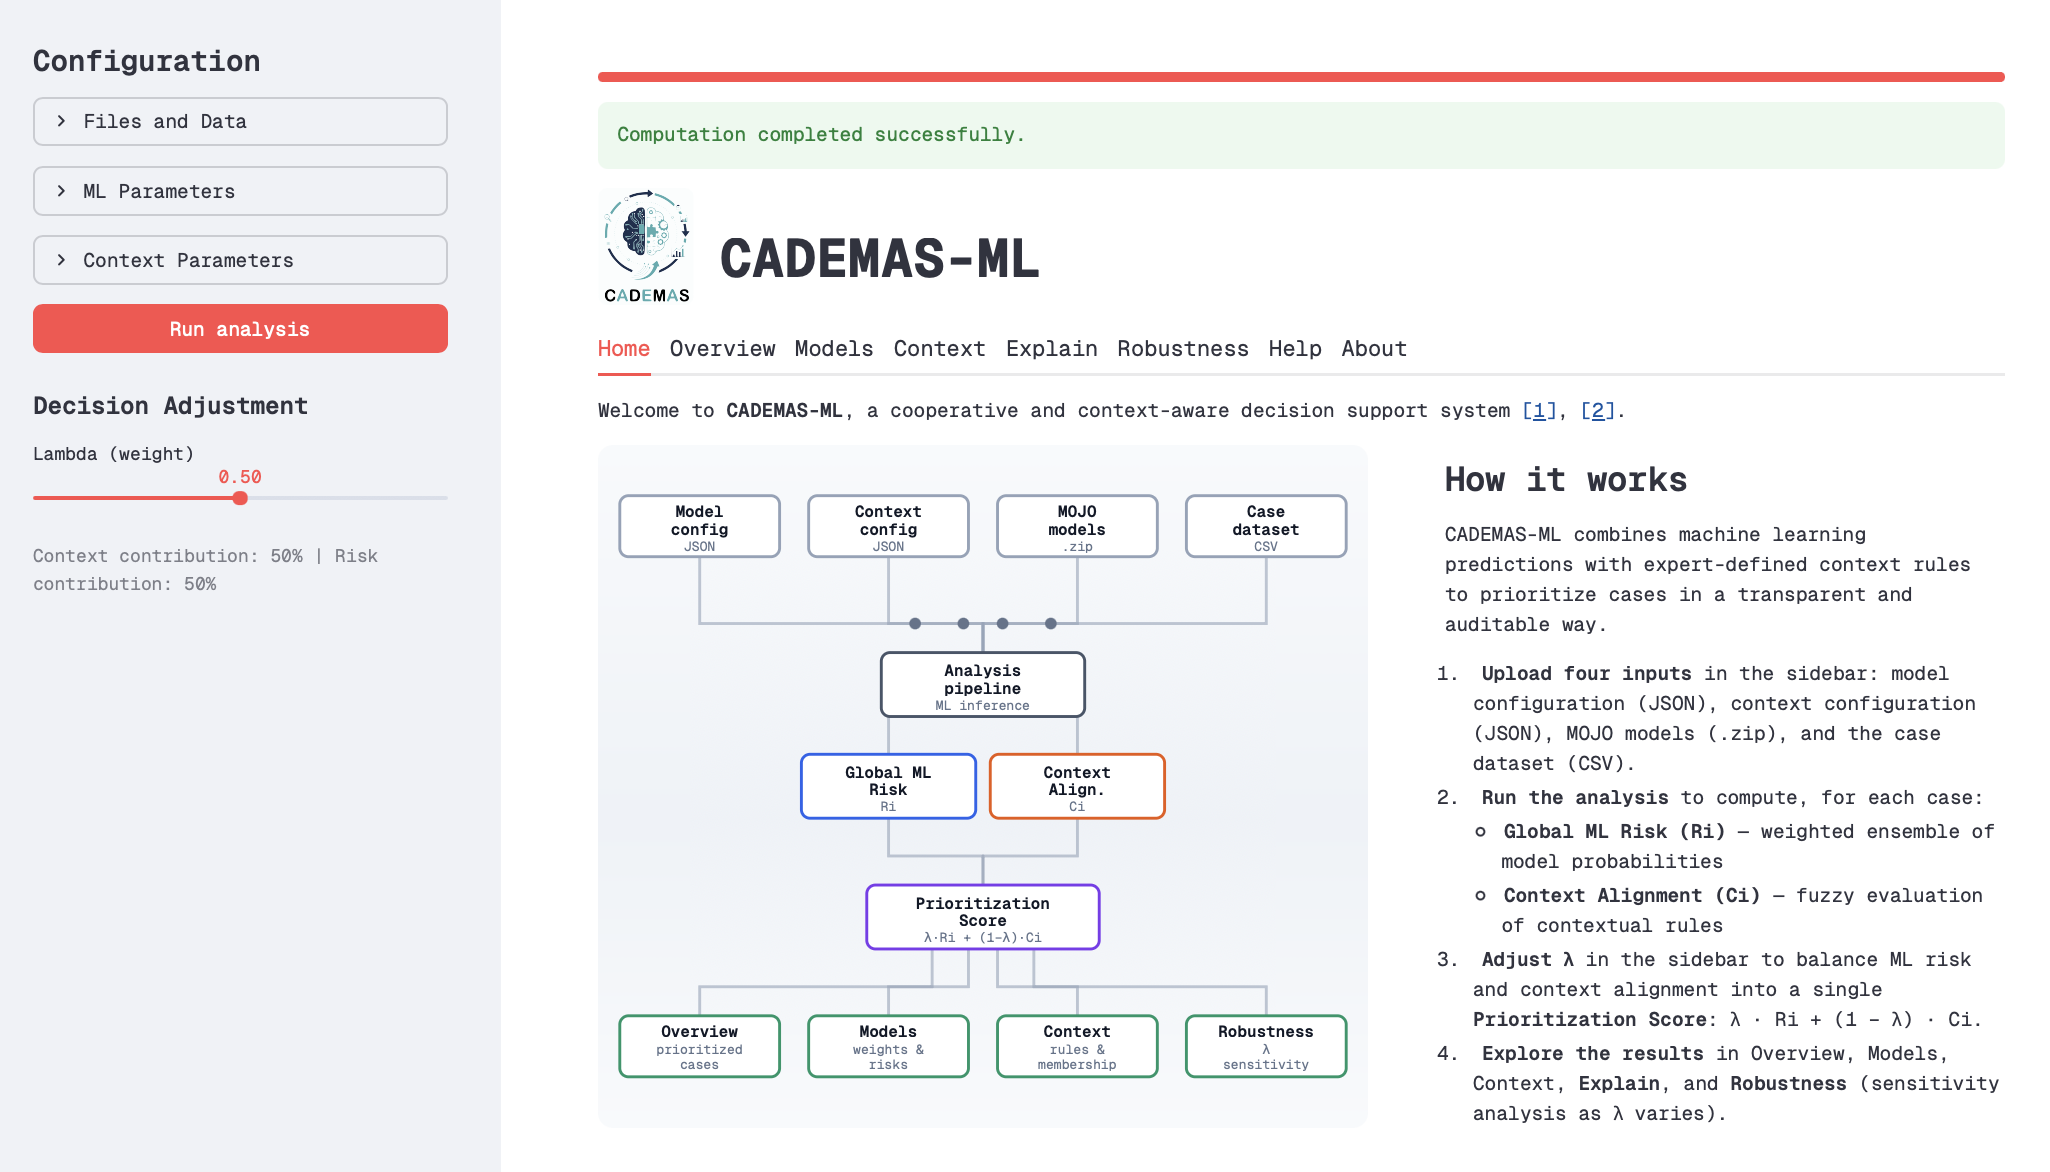
\includegraphics[width=\textwidth,height=0.34\textheight,keepaspectratio]{figures/home.png}
\caption{\textit{Home} and input configuration module. The user uploads or loads the four inputs and launches the analysis pipeline described in Section~\ref{sec:implementation}.}
\label{fig:home_upload}
\end{figure}

The user provides the four inputs required by the architecture---model-metadata JSON, context JSON, MOJO models, and the case dataset---or loads the ready-made example distributed under \texttt{example\_attrition/}\footnote{\url{https://github.com/pnovoa/cademas-app/tree/main/example_attrition}.}. The application \textit{Help} panel documents the same bundle. Before execution, the user selects the validation metric used for model weighting, chooses one of the uploaded context specifications, sets the balance parameter $\lambda$, and triggers \textit{Run analysis}. CADEMAS-ML then executes the pipeline defined in Section~\ref{sec:implementation}: MOJO inference, fuzzy context evaluation, and score integration. Table~\ref{tab:tool_model_weights} summarizes the four pre-trained ADM units included in the example and the AUC-based weights recomputed during the run.

\begin{table}[!t]
\tbl{Models used in the attrition example and AUC-based weights computed by CADEMAS-ML. The \textit{AutoML model} column summarizes the artifact exported by H2O AutoML.}
{\footnotesize
\begin{tabularx}{\textwidth}{lllcc}
\toprule
\textbf{ID} & \textbf{Organizational perspective} & \textbf{AutoML model} & \textbf{AUC} & \textbf{Weight} \\
\midrule
$M_1$ & Culture and Wellbeing & Stacked Ensemble (BestOfFamily) & 0.9941 & 0.2623 \\
$M_2$ & Finance & Stacked Ensemble (BestOfFamily) & 0.9972 & 0.2631 \\
$M_3$ & Operations and Development & GBM (grid 1, model 26) & 0.8022 & 0.2116 \\
$M_4$ & Human Resources & Stacked Ensemble (BestOfFamily) & 0.9968 & 0.2630 \\
\bottomrule
\end{tabularx}}
\label{tab:tool_model_weights}
\end{table}

Following the training protocol of \citet{Godz2026}, the four MOJO models correspond to the organizational perspectives summarized in Table~\ref{tab:tool_model_weights}. Using AUC as the weighting metric, the reproduced run assigns a lower weight to Operations and Development because its validation AUC is lower than that of the other three components.

\section{Results}\label{sec:results}

This section follows the analysis path exposed by the application. It first reports the integrated ranking, then examines the predictive and contextual components separately, and finally presents case-level explanations and ranking sensitivity. Unless otherwise stated, all outputs correspond to the \textit{Digital / Technological Transformation} context, AUC-based model weights, and $\lambda=0.5$ defined in Section~\ref{sec:demonstration}.

\subsection{\textit{Overview}: integrated prioritization}

After execution, the \textit{Overview} module surfaces the outputs of Equations~\eqref{eq:ml_risk}--\eqref{eq:priority_lambda}. Figure~\ref{fig:overview} shows the exported interface. At the top, the \textit{Prioritization: Risk vs Context} scatter plot locates each case in the $(R_i,C_i)$ plane and encodes $P_i(0.5)$ through color; the adjacent \textit{Prioritization Score} histogram summarizes the cohort-wide distribution of prioritization scores. Below, the \textit{Prioritized Cases} table lists all cases ordered by $P_i(0.5)$, reporting $R_i$, $C_i$, and the \texttt{attrition} outcome label retained for verification only. In this run, $C_i$ ranges from 0.1500 to 0.7100, with a mean of 0.4663. The ten highest-priority cases at $\lambda=0.5$ are used later in the robustness analysis of Figure~\ref{fig:robustness}.

\begin{figure}[!tb]
\centering 
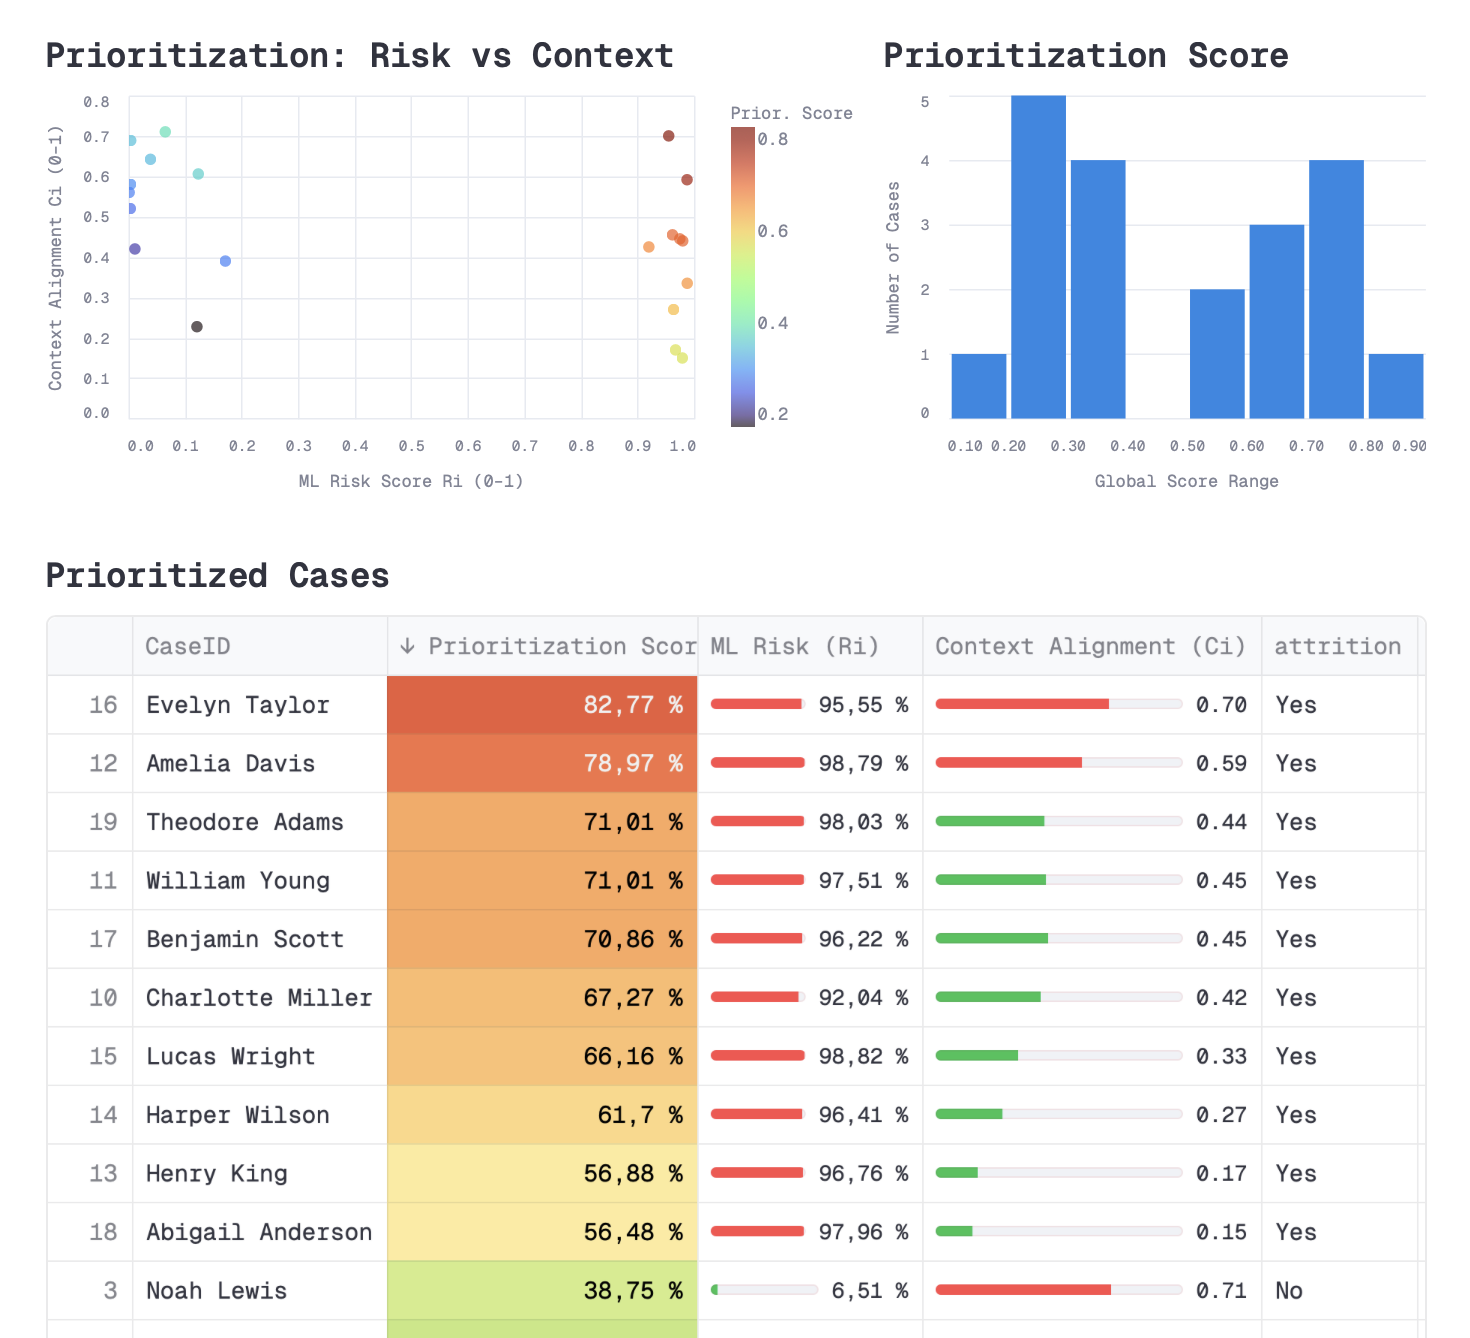
\includegraphics[width=\textwidth]{figures/overview.png}
\caption{\textit{Overview} module for the attrition example at $\lambda=0.5$ in the \textit{Digital / Technological Transformation} context. The scatter plot and histogram summarize the risk--context landscape and the distribution of $P_i(0.5)$; the \textit{Prioritized Cases} table below lists the full cohort by prioritization score, including high-priority employees and context-aligned but low-risk cases such as \textit{Noah Lewis}.}
\label{fig:overview}
\end{figure}

The prioritization ranking in Figure~\ref{fig:overview} is driven primarily by cooperative predictive risk. The highest-priority cases exhibit high $R_i$, while $C_i$ varies more widely. \textit{Evelyn Taylor} leads the ranking because both components are high ($R_i=0.9555$, $C_i=0.7000$), producing $P_i(0.5)=0.8277$. Cases such as \textit{Lucas Wright} and \textit{Abigail Anderson} remain near the top mainly because of critical predictive risk, even though their contextual alignment is moderate or low. By contrast, \textit{Noah Lewis} appears far down the table despite having the highest $C_i$ in the cohort ($C_i=0.7100$): his cooperative predictive risk is low ($R_i=0.0651$), yielding $P_i(0.5)=0.3875$. The juxtaposition of scatter plot, score distribution, and full case table illustrates why CADEMAS-ML reports $P_i(\lambda)$, $R_i$, and $C_i$ separately rather than ranking cases by contextual alignment alone.

\subsection{\textit{Models}: cooperative predictive risk}

The \textit{Models} module exposes the intermediate results of the cooperative predictive-risk layer defined in Equation~\eqref{eq:ml_risk}. Figure~\ref{fig:models} shows the exported interface for the reproduced run. The upper table, \textit{Model Weights}, links each uploaded MOJO to its normalized contribution $w_k$; the values displayed are consistent with those reported in Table~\ref{tab:tool_model_weights}. The lower table, \textit{Risk Probabilities}, reports the per-case positive-class probability returned by each model and the cooperative score $R_i$ in the column immediately after \texttt{CaseID}; cases are ordered by decreasing $R_i$.

\begin{figure}[!tb]
\centering
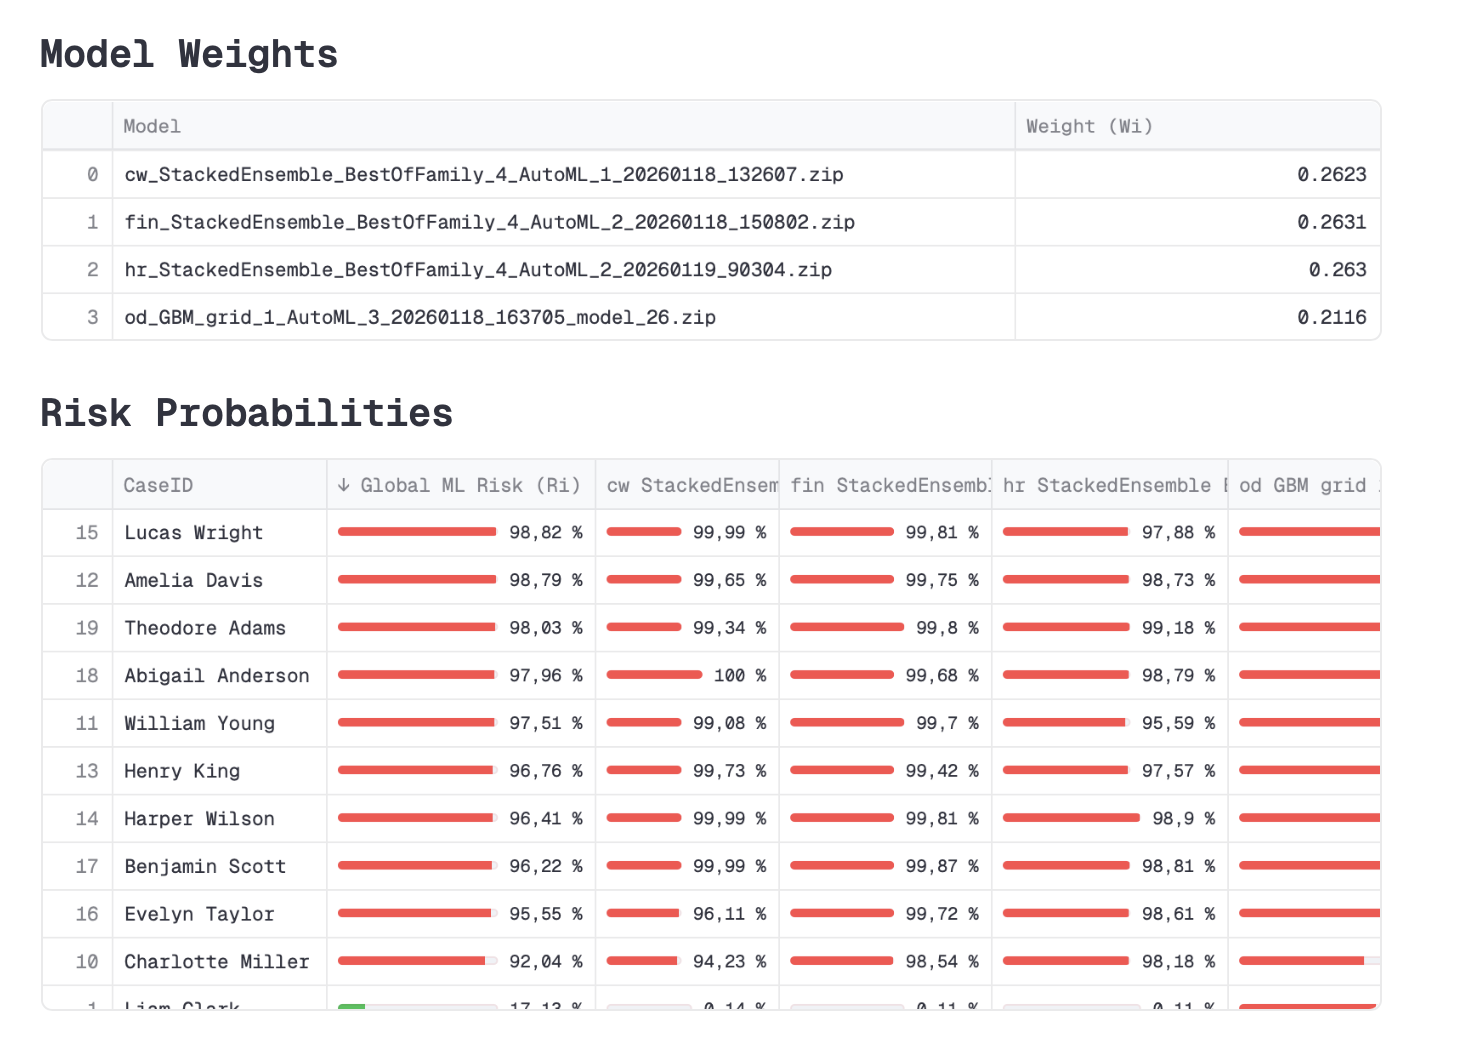
\includegraphics[width=\textwidth]{figures/models.png}
\caption{\textit{Models} module for the attrition example, showing the model-weight table that assigns each MOJO its contribution $w_k$ and, below, the risk-probability table with Global ML Risk ($R_i$), per-model probabilities, and cases sorted by decreasing $R_i$.}
\label{fig:models}
\end{figure}

In the exported view, \textit{Lucas Wright} appears first ($R_i=0.9882$), followed by \textit{Amelia Davis} ($R_i=0.9879$) and \textit{Theodore Adams} ($R_i=0.9803$). This ordering differs from the integrated prioritization in Figure~\ref{fig:overview}, where \textit{Evelyn Taylor} leads because $P_i(0.5)$ also incorporates contextual alignment. The side-by-side per-model columns make the cooperative aggregation auditable: although all four MOJOs assign high attrition probabilities to the top rows, Operations and Development contributes less to $R_i$ because its validation weight is lower ($w_3=0.2116$, consistent with Table~\ref{tab:tool_model_weights}). Together, the two tables connect the model-confidence layer of Equation~\eqref{eq:model_weights} to the case-level cooperative predictive risk fed into the prioritization score.

\subsection{\textit{Context}: contextual alignment}

The \textit{Context} module renders the fuzzy audit underlying Equation~\eqref{eq:context_score}. Figure~\ref{fig:context} exports the interface for the \textit{Digital / Technological Transformation} context. The upper panel lets analysts select an atomic rule and inspect its membership function together with the cohort distribution of the underlying feature; a \textit{Numerical Audit} table on the right reports, for each case, the crisp input value and the corresponding membership degree $\mu$. The lower panel, \textit{Derived Rules Overview}, summarizes satisfaction in the composite rules and the resulting context-alignment score $C_i$ for the full cohort.  

\begin{figure}[!tb]
\centering
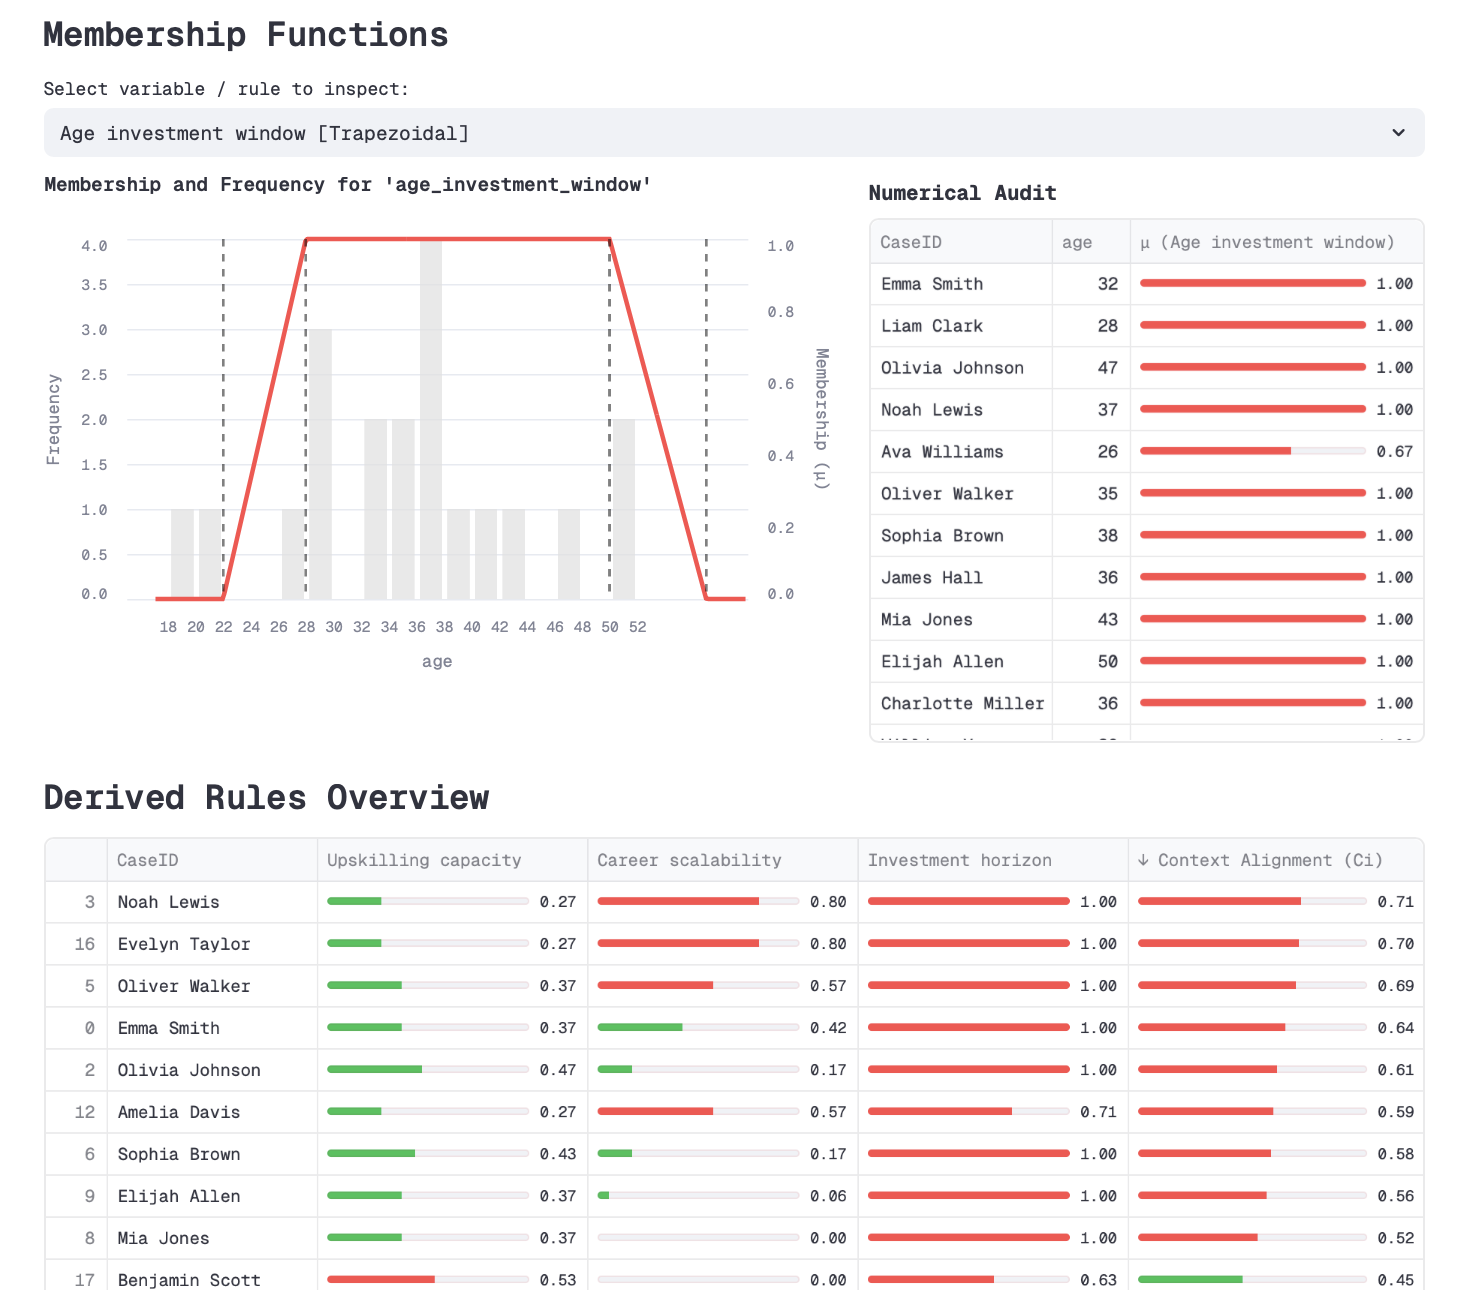
\includegraphics[width=\textwidth]{figures/context.png}
\caption{\textit{Context} module for the \textit{Digital / Technological Transformation} run, combining an atomic-rule selector, the membership-function chart with case distribution, and the numerical audit table for \textit{Age investment window} (trapezoidal), together with a derived-rules overview reporting membership degrees and $C_i$ for cases ordered by decreasing context alignment.}
\label{fig:context}
\end{figure}

In the exported view, the analyst has selected the trapezoidal atomic rule \textit{Age investment window}, which defines the acceptable age range for developmental investment during the transformation program (Appendix~\ref{app:context_specs}). The chart links each employee's age to its membership $\mu$, while the audit table makes the same mapping explicit case by case. Below, \textit{Derived Rules Overview} exposes the degrees of satisfaction for \textit{Upskilling capacity}, \textit{Career scalability}, and \textit{Investment horizon}, together with the aggregated score $C_i$. The table is sorted by $C_i$ in descending order, so \textit{Noah Lewis} ($C_i=0.7100$) appears first and \textit{Evelyn Taylor} ($C_i=0.7000$) second, even though Evelyn leads the integrated ranking in Figure~\ref{fig:overview} because of higher cooperative risk. This view therefore complements the prioritization summary by making the contextual evidence auditable rule by rule and case by case.

\subsection{\textit{Explain}: local case interpretation}

For a selected case, the \textit{Explain} module assembles the four explanation levels defined in Section~\ref{sec:implementation} into a single audit view. Figure~\ref{fig:explain} exports the interface for \textit{Evelyn Taylor}, the highest-priority case in Figure~\ref{fig:overview}. Figure~\ref{fig:explain}-A shows the case selector, the deterministic natural-language summary, and the headline statistics on which that summary rests: $P_i(0.5)$, $R_i$, $C_i$, and $\lambda$, together with the additive decomposition in Equation~\eqref{eq:priority_decomposition}. Figure~\ref{fig:explain}-B reports the aggregated ML attributions for the ten most influential features and, below, the fuzzy memberships that trace how strongly each contextual rule is satisfied for the selected case.

\begin{figure}[!tb]
\centering
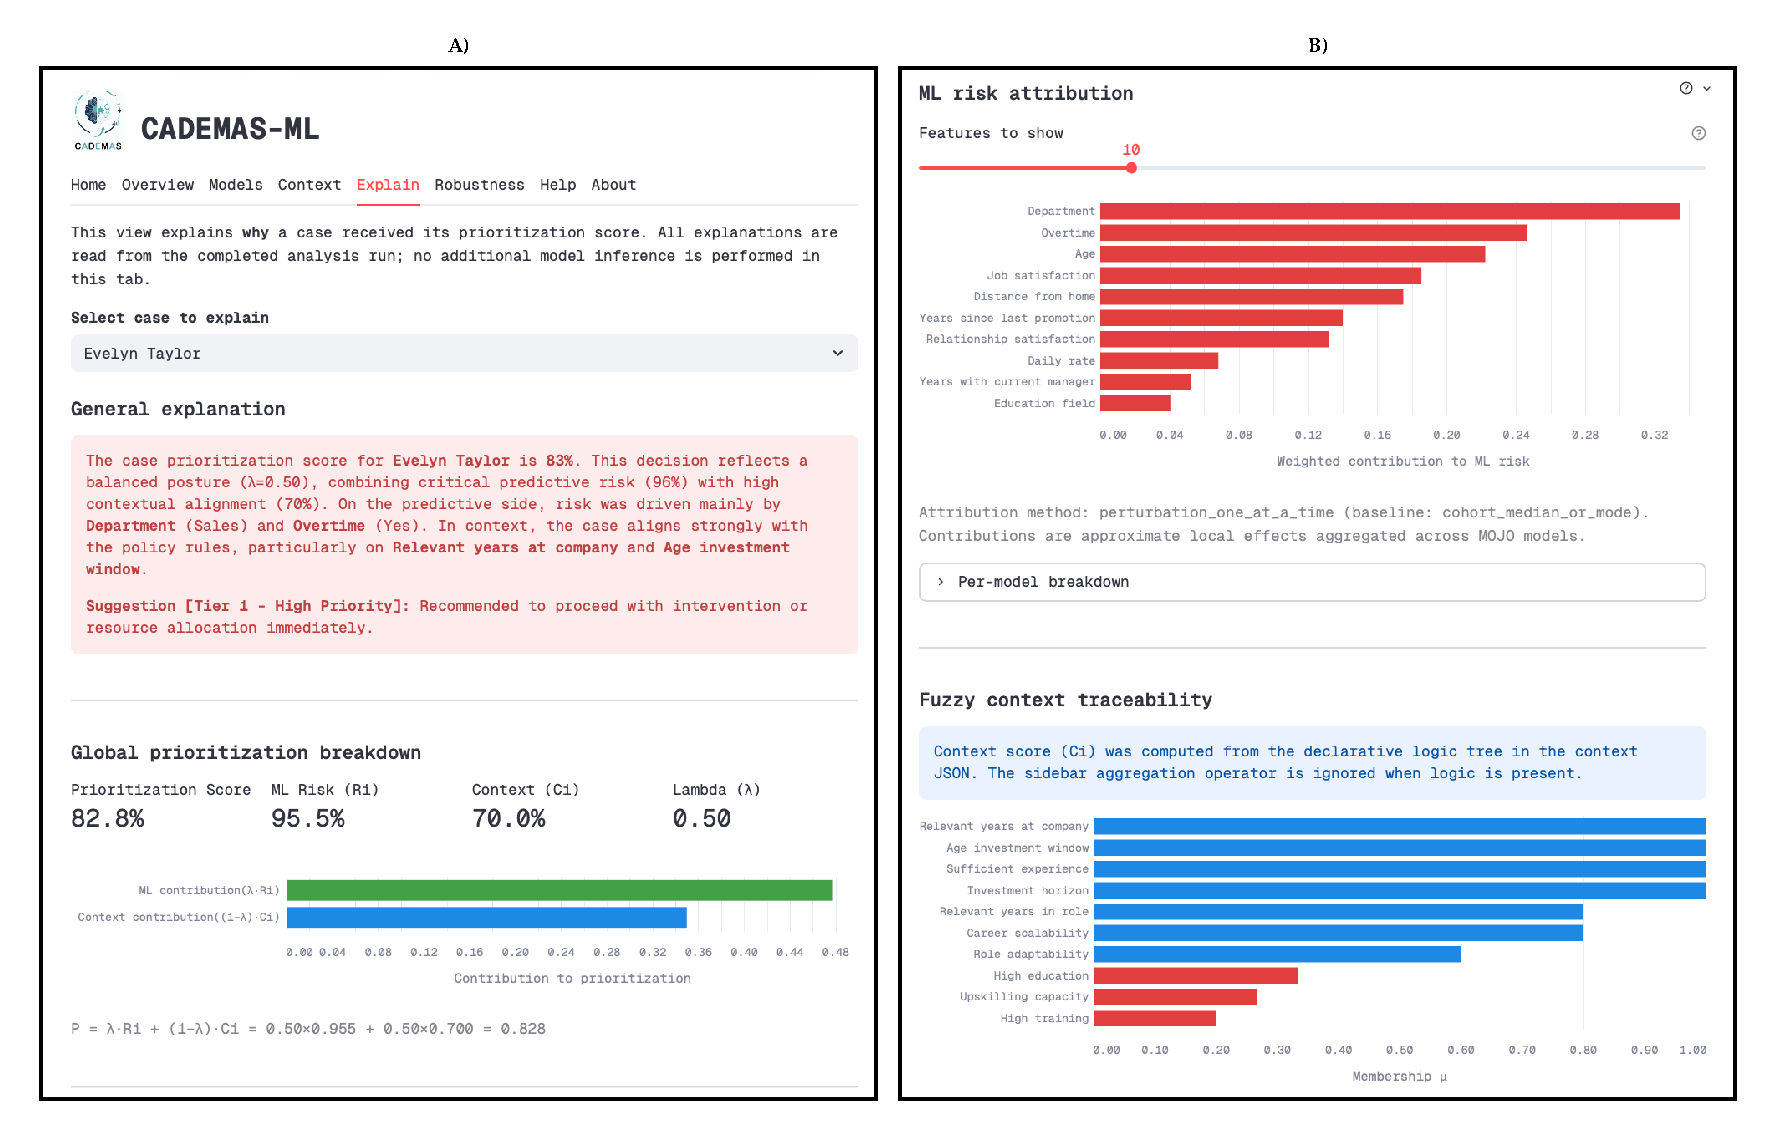
\includegraphics[width=\textwidth]{figures/explain_high_prioritization.pdf}
\caption{\textit{Explain} module for \textit{Evelyn Taylor} at $\lambda=0.5$ in the \textit{Digital / Technological Transformation} context, with case selection, natural-language explanation, summary statistics, aggregated bar charts of the ten most influential ML features, and a fuzzy context traceability panel reporting membership degrees for the policy rules.}
\label{fig:explain}
\end{figure}

Two cases illustrate the interpretation produced by the \textit{Explain} module. The first is \textit{Evelyn Taylor}, ranked first in Figure~\ref{fig:overview} and reproduced in Figure~\ref{fig:explain}; the second is \textit{Noah Lewis}, who ranks low in the same overview despite having the highest $C_i$ in the cohort. For space reasons, only the \textit{Evelyn Taylor} view is shown in the figure; the contrasting \textit{Noah Lewis} summary is reported below in textual form. In both cases, the summaries were reproduced from CADEMAS-ML and follow its deterministic template: $P_i(\lambda)$ is reported first, followed by $\lambda$, the levels of $R_i$ and $C_i$, the main ML drivers, the contextual rules that support or constrain priority, and the tier-based recommendation.

\textit{Evelyn Taylor} combines critical predictive risk ($R_i=0.9555$) with high contextual alignment ($C_i=0.7000$), yielding $P_i(0.5)=0.8277$ and a \textit{Tier 1} recommendation. Figure~\ref{fig:explain}-A displays these values together with the natural-language synthesis; Figure~\ref{fig:explain}-B highlights Department (Sales) and Overtime (Yes) among the strongest ML drivers and shows high membership on Relevant years at company and Age investment window in the fuzzy traceability panel:

\begin{quote} 
\small
The case prioritization score for \textit{Evelyn Taylor} is 83\%. This decision reflects a balanced posture ($\lambda=0.50$), combining critical predictive risk (96\%) with high contextual alignment (70\%). On the predictive side, risk was driven mainly by Department (Sales) and Overtime (Yes). In context, the case aligns strongly with the policy rules, particularly on Relevant years at company and Age investment window.

Suggestion [\textit{Tier 1} -- High Priority]: Recommended to proceed with intervention or resource allocation immediately.
\end{quote} 

\textit{Noah Lewis} provides a contrasting interpretation. Although this case has the highest contextual alignment in the cohort ($C_i=0.7100$), its cooperative predictive risk is low ($R_i=0.0651$). The resulting prioritization score is therefore $P_i(0.5)=0.3875$, and the module assigns \textit{Tier 3}:

\begin{quote}
\small
The case prioritization score for \textit{Noah Lewis} is 39\%. This decision reflects a balanced posture ($\lambda=0.50$), combining low predictive risk (7\%) with high contextual alignment (71\%). On the predictive side, risk was driven mainly by Years with current manager (8) and Number of companies worked (1). In context, the case aligns strongly with the policy rules, particularly on Relevant years at company and Age investment window.

Suggestion [\textit{Tier 3} -- Low Priority]: Intervention or resource allocation is not justified under current prediction and context guidelines.
\end{quote}

In practical terms, CADEMAS-ML explains not only why a case is prioritized, but also why another case with strong contextual alignment may still receive a low final score when predictive risk remains limited. A third illustrative pattern is provided by \textit{Theodore Adams} ($R_i=0.9803$, $C_i=0.4400$, $P_i(0.5)=0.7101$), who receives \textit{Tier 2} because high predictive risk and only moderate contextual alignment produce borderline evidence under the current policy.

\subsection{\textit{Robustness}: sensitivity of the priority ranking}

The \textit{Robustness} module implements the sensitivity analysis defined in Section~\ref{sec:implementation}. Figure~\ref{fig:robustness} illustrates the exported Altair charts using $\Lambda=\{0,0.25,0.5,0.75,1\}$ and the ten highest-priority cases at $\lambda=0.5$ (the head of the ranking in Figure~\ref{fig:overview}).

Figure~\ref{fig:robustness}-A shows the bump chart of priority ranks across $\lambda$. Figure~\ref{fig:robustness}-B reports the ranks box plot, which summarizes the rank distribution of each displayed case over the same sweep; cases are ordered from left to right by median rank and, in case of ties, by interquartile range. Figure~\ref{fig:robustness}-C shows the rank acceptability indices, estimating the relative frequency with which each case occupies each rank position over $\Lambda$.

\begin{figure}[!htb]
  \centering
  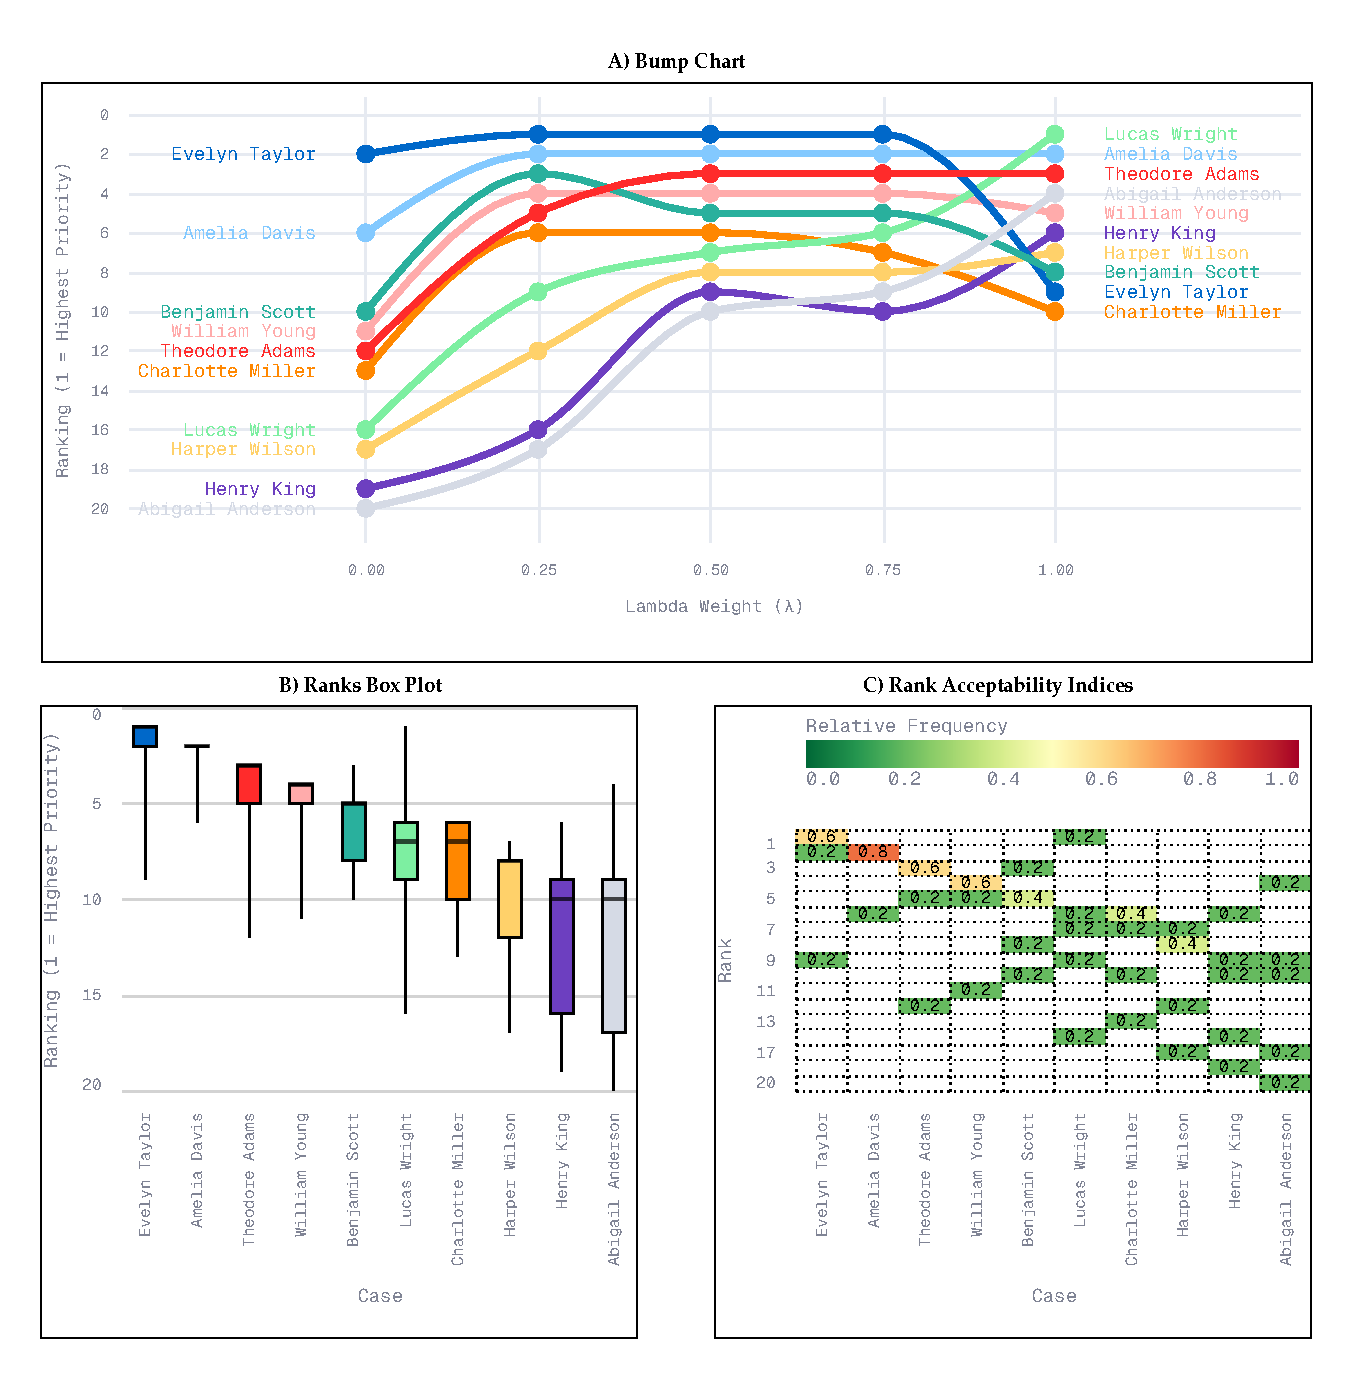
\includegraphics[width=\textwidth]{figures/robustness.pdf}
  \caption{Robustness analysis for the \textit{Digital / Technological Transformation} context exported from CADEMAS-ML over $\Lambda=\{0,0.25,0.5,0.75,1\}$ for the ten highest-priority cases at $\lambda=0.5$, comprising a bump chart of priority ranks across $\lambda$, a ranks box plot of rank distributions over the same sweep, and rank acceptability indices.}
  \label{fig:robustness}
\end{figure}

When $\lambda$ approaches 0 and contextual alignment receives greater weight, cases outside the top ten at $\lambda=0.5$, such as \textit{Noah Lewis} and \textit{Emma Smith}, rise in Figure~\ref{fig:robustness}-A because they combine high $C_i$ with low $R_i$. When $\lambda$ approaches 1, the high-risk cases at the head of Figure~\ref{fig:overview}---such as \textit{Lucas Wright} and \textit{Theodore Adams}---dominate the ranking regardless of transformation alignment. \textit{Evelyn Taylor} remains near the top across intermediate values of $\lambda$ because both $R_i$ and $C_i$ are high. The box plot in Figure~\ref{fig:robustness}-B makes this contrast visible at a glance: stable high-priority cases exhibit compact rank distributions, whereas policy-sensitive cases show wider spreads. Figure~\ref{fig:robustness}-C complements both views by quantifying how often each case attains each rank over the $\lambda$ grid.

\section{Discussion}\label{sec:discussion}

This paper presented CADEMAS-ML as an executable specialization of the CADEMAS framework for cooperative, context-aware, ML-based prioritization. Its contribution is not a new attrition predictor, but an operational separation of predictive evidence, contextual evaluation, and final prioritization. This separation builds on the general architecture of \citet{NovoaHernandez2026} and the employee-attrition instantiation of \citet{Godz2026}, while adding reusable configuration, case-level explanation, and ranking-sensitivity analysis. The employee-attrition demonstration shows the practical consequence of that design: rankings based on cooperative predictive risk need not coincide with rankings based on contextual alignment, and the explicit combination of both can be inspected rather than treated as an opaque post-processing step.

The tool also occupies a distinct position relative to related decision-support software. Existing platforms and libraries have made important advances in exposing intermediate fuzzy or multi-criteria calculations \citep{Wieckowski2024,Chekry2024}, while hybrid approaches have combined prediction, ranking, expert knowledge, and explainability in application-specific pipelines \citep{Ozkurt2025}. CADEMAS-ML complements these contributions by organizing the workflow around cooperating ADM units and by keeping their integrated output separate from the context in which a decision is made. The \textit{Models}, \textit{Context}, and \textit{Overview} views preserve this distinction; the \textit{Explain} and \textit{Robustness} views then support case-level interpretation and policy-sensitivity analysis. These additions extend the static prioritization workflow considered in earlier CADEMAS work.

For practitioners, the main benefit of this architecture is the ability to revise decision policy without embedding that policy in the predictive models themselves. When organizational conditions change, analysts can retain the predictive layer, provide a different context specification, and examine how the resulting priorities change. The separate reporting of $R_i$, $C_i$, and $P_i(\lambda)$ makes the source of a recommendation visible, while the $\lambda$ sweep identifies cases whose position is stable and cases whose priority depends strongly on the selected balance. This does not remove the need for professional judgment; rather, it provides a structured record of the predictive and policy assumptions presented to the decision-maker. Potential applications include alert triage, review queues, retention programs, and allocation of limited support or inspection resources, provided that models, contextual rules, and decision thresholds are validated for the domain concerned.

For researchers, CADEMAS-ML provides a reproducible environment in which alternative cooperation, context-representation, explanation, and robustness mechanisms can be compared within a common architecture. The current implementation uses performance-normalized weights to combine independently trained models and a convex linear rule, $P_i(\lambda)=\lambda R_i+(1-\lambda)C_i$, to integrate predictive risk and context. This final rule is compensatory: sufficiently strong evidence in one component can offset weaker evidence in the other. Recent work on aggregation semantics for CADEMAS \citep{novoa2026aggregation} motivates extending the software with operator families that express different compensation requirements, including conjunctive or veto-like behavior. Making the aggregation semantics configurable would allow the software to distinguish settings in which compensation is acceptable from those in which a minimum level of predictive or contextual support is required.

A related direction is to move cooperation upstream, from post-hoc output aggregation to model development. At present, the predictive ADM units are trained independently and cooperation begins when their probabilities are weighted. Future versions could investigate diversity-aware model selection, theory-informed learning constraints, or multi-objective procedures that balance predictive performance, calibration, and complementarity. The aim would not be to encourage disagreement for its own sake, but to obtain models that remain individually reliable while contributing non-redundant evidence from different variables, data sources, or perspectives on the problem. Measures of conditional competence and redundancy could then inform both training and aggregation, providing a more principled trade-off between the performance of individual ADM units and the informational value of their cooperation.

Several limitations delimit these implications. The ADM units currently supported at run time are H2O MOJO classifiers; the broader CADEMAS notion of heterogeneous units, including optimization models, simulators, or rule-based systems, is not yet implemented. Local ML attributions are model-agnostic perturbations around a cohort baseline and should not be read as causal effects or as substitutes for model-specific explanation methods when model internals are available. The attrition demonstration uses a 20-case illustrative subset and is neither a predictive-performance study nor evidence for general human-resources policy. Moreover, context specifications require domain-expert elicitation, and the interface does not yet provide versioned approval workflows or immutable audit trails for production governance. Future development should therefore combine broader ADM support and richer aggregation semantics with empirical validation in additional domains, stronger context governance, and evaluation with the practitioners who would interpret and act on the resulting priorities.

\section*{Funding}

This research was supported by the project ``Study, Analysis and Evaluation of Cooperative Automated Decision-Making Systems (CADEMAS)'', PID2023-146575NB-I00, funded by MCIU/AEI/10.13039/501100011033 and by FEDER, EU.

\section*{Disclosure statement}

The authors report there are no competing interests to declare.

\section*{Declaration of generative AI use}

Generative AI tools were used to assist with language editing and manuscript formatting. The authors reviewed and take full responsibility for the content of this article.

\section*{Data availability statement}

The illustrative employee records used in this article are a 20-case subset derived from the publicly available IBM HR Analytics Employee Attrition and Performance dataset \citep{IBMHRKaggle}. The subset, model metadata, MOJO archives, and context specifications are distributed with the software repository cited in Section~\ref{sec:software}.

\phantomsection
\section*{Software availability}\label{sec:software}

CADEMAS-ML is available at \url{https://github.com/pnovoa/cademas-app} under an MIT license \citep{cademasml2026}. An archival snapshot will be deposited in Zenodo at the time of submission; the corresponding DOI will be inserted when it is available.

\section*{Supplementary material}

Supplementary Material~S1 accompanies this article and provides the complete specification of the four application inputs, field-level constraints, cross-file consistency requirements, and minimal configuration examples.

\section*{Author contributions}

Pavel Novoa-Hern\'{a}ndez: conceptualization, methodology, software, validation, writing -- original draft, visualization. David A. Pelta: conceptualization, methodology, supervision, writing -- review and editing.

\begin{thebibliography}{}

\bibitem [\protect \citeauthoryear {%
Abdulgader%
, Eid%
\BCBL {}\ \BBA {} Daneshvar~Rouyendegh%
}{%
Abdulgader%
\ \protect \BOthers {.}}{%
{\protect \APACyear {2018}}%
}]{%
Abdulgader2018}
\APACinsertmetastar {%
Abdulgader2018}%
\begin{APACrefauthors}%
Abdulgader, F\BPBI S.%
, Eid, R.%
\BCBL {}\ \BBA {} Daneshvar~Rouyendegh, B.%
\end{APACrefauthors}%
\unskip\
\newblock
\APACrefYearMonthDay{2018}{{\APACmonth{11}}}{}.
\newblock
{\BBOQ}\APACrefatitle {Development of Decision Support Model for Selecting a
  Maintenance Plan Using a Fuzzy {MCDM} Approach: A Theoretical Framework}
  {Development of decision support model for selecting a maintenance plan using
  a fuzzy {MCDM} approach: A theoretical framework}.{\BBCQ}
\newblock
\APACjournalVolNumPages{Applied Computational Intelligence and Soft
  Computing}{2018}{}{1--14}.
\newblock
\begin{APACrefDOI} \doi{10.1155/2018/9346945} \end{APACrefDOI}
\PrintBackRefs{\CurrentBib}

\bibitem [\protect \citeauthoryear {%
Barredo~Arrieta%
\ \protect \BOthers {.}}{%
Barredo~Arrieta%
\ \protect \BOthers {.}}{%
{\protect \APACyear {2020}}%
}]{%
Arrieta2020}
\APACinsertmetastar {%
Arrieta2020}%
\begin{APACrefauthors}%
Barredo~Arrieta, A.%
, D{\'i}az-Rodr{\'i}guez, N.%
, Del~Ser, J.%
, Bennetot, A.%
, Tabik, S.%
, Barbado, A.%
\BDBL {}Herrera, F.%
\end{APACrefauthors}%
\unskip\
\newblock
\APACrefYearMonthDay{2020}{{\APACmonth{06}}}{}.
\newblock
{\BBOQ}\APACrefatitle {Explainable {Artificial Intelligence} ({XAI}): Concepts,
  Taxonomies, Opportunities and Challenges Toward Responsible {AI}}
  {Explainable {Artificial Intelligence} ({XAI}): Concepts, taxonomies,
  opportunities and challenges toward responsible {AI}}.{\BBCQ}
\newblock
\APACjournalVolNumPages{Information Fusion}{58}{}{82--115}.
\newblock
\begin{APACrefDOI} \doi{10.1016/j.inffus.2019.12.012} \end{APACrefDOI}
\PrintBackRefs{\CurrentBib}

\bibitem [\protect \citeauthoryear {%
Borkotokey%
, Hazarika%
\BCBL {}\ \BBA {} Mesiar%
}{%
Borkotokey%
\ \protect \BOthers {.}}{%
{\protect \APACyear {2019}}%
}]{%
Borkotokey2019}
\APACinsertmetastar {%
Borkotokey2019}%
\begin{APACrefauthors}%
Borkotokey, S.%
, Hazarika, P.%
\BCBL {}\ \BBA {} Mesiar, R.%
\end{APACrefauthors}%
\unskip\
\newblock
\APACrefYearMonthDay{2019}{{\APACmonth{09}}}{}.
\newblock
{\BBOQ}\APACrefatitle {Cooperative Games with Multiple Attributes} {Cooperative
  games with multiple attributes}.{\BBCQ}
\newblock
\APACjournalVolNumPages{International Journal of General
  Systems}{48}{8}{825--842}.
\newblock
\begin{APACrefDOI} \doi{10.1080/03081079.2019.1659792} \end{APACrefDOI}
\PrintBackRefs{\CurrentBib}

\bibitem [\protect \citeauthoryear {%
Chekry%
\ \protect \BOthers {.}}{%
Chekry%
\ \protect \BOthers {.}}{%
{\protect \APACyear {2024}}%
}]{%
Chekry2024}
\APACinsertmetastar {%
Chekry2024}%
\begin{APACrefauthors}%
Chekry, A.%
, Bakkas, J.%
, Hanine, M.%
, Montero, E\BPBI C.%
, {Garat de Marin}, M\BPBI S.%
\BCBL {}\ \BBA {} Ashraf, I.%
\end{APACrefauthors}%
\unskip\
\newblock
\APACrefYearMonthDay{2024}{}{}.
\newblock
{\BBOQ}\APACrefatitle {{PyDEMATEL}: A {Python}-based tool implementing
  {DEMATEL} and fuzzy {DEMATEL} methods for improved decision making}
  {{PyDEMATEL}: A {Python}-based tool implementing {DEMATEL} and fuzzy
  {DEMATEL} methods for improved decision making}.{\BBCQ}
\newblock
\APACjournalVolNumPages{SoftwareX}{}{}{}.
\newblock
\begin{APACrefDOI} \doi{10.1016/j.softx.2024.101889} \end{APACrefDOI}
\PrintBackRefs{\CurrentBib}

\bibitem [\protect \citeauthoryear {%
Deliu%
\ \BBA {} Moldovan%
}{%
Deliu%
\ \BBA {} Moldovan%
}{%
{\protect \APACyear {2026}}%
}]{%
Deliu2026}
\APACinsertmetastar {%
Deliu2026}%
\begin{APACrefauthors}%
Deliu, D.%
\BCBT {}\ \BBA {} Moldovan, A\BHBI L.%
\end{APACrefauthors}%
\unskip\
\newblock
\APACrefYearMonthDay{2026}{}{}.
\newblock
{\BBOQ}\APACrefatitle {Human--{AI} Collaboration and Cognitive Flexibility in
  Industry 6.0: A Framework for Purposeful Decision-Making in Innovation and
  Project Management} {Human--{AI} collaboration and cognitive flexibility in
  industry 6.0: A framework for purposeful decision-making in innovation and
  project management}.{\BBCQ}
\newblock
\APACjournalVolNumPages{International Journal of Managing Projects in
  Business}{}{}{}.
\newblock
\begin{APACrefDOI} \doi{10.1108/ijmpb-10-2025-0459} \end{APACrefDOI}
\PrintBackRefs{\CurrentBib}

\bibitem [\protect \citeauthoryear {%
{European Law Institute}%
}{%
{European Law Institute}%
}{%
{\protect \APACyear {2022}}%
}]{%
EIP2022}
\APACinsertmetastar {%
EIP2022}%
\begin{APACrefauthors}%
{European Law Institute}.%
\end{APACrefauthors}%
\unskip\
\newblock
\APACrefYearMonthDay{2022}{}{}.
\newblock
\APACrefbtitle {{Guiding Principles for Automated Decision-Making in the EU}}
  {{Guiding Principles for Automated Decision-Making in the EU}}\ \APACbVolEdTR
  {}{ELI Innovation Paper}.
\newblock
\APACaddressInstitution{}{{European Law Institute (ELI)}}.
\newblock
\APACrefnote{ISBN 978-3-9505192-7-3. Available at
  \url{https://www.europeanlawinstitute.eu/fileadmin/user_upload/p_eli/Publications/ELI_Innovation_Paper_on_Guiding_Principles_for_ADM_in_the_EU.pdf}
  (accessed 15 January 2026)}
\PrintBackRefs{\CurrentBib}

\bibitem [\protect \citeauthoryear {%
Godz%
, Novoa-Hernández%
\BCBL {}\ \BBA {} Pelta%
}{%
Godz%
\ \protect \BOthers {.}}{%
{\protect \APACyear {2026}}%
}]{%
Godz2026}
\APACinsertmetastar {%
Godz2026}%
\begin{APACrefauthors}%
Godz, M.%
, Novoa-Hernández, P.%
\BCBL {}\ \BBA {} Pelta, D\BPBI A.%
\end{APACrefauthors}%
\unskip\
\newblock
\APACrefYearMonthDay{2026}{}{}.
\newblock
{\BBOQ}\APACrefatitle {A Cooperative and Context-Aware Approach for Employee
  Attrition Prevention} {A cooperative and context-aware approach
  for employee attrition prevention}.{\BBCQ}
\newblock
\BIn{} \APACrefbtitle {Information Processing and Management of Uncertainty in
  Knowledge-Based Systems} {Information processing and management of
  uncertainty in knowledge-based systems}\ (\BPGS\ 203--217).
\newblock
\APACaddressPublisher{}{Springer Nature Switzerland}.
\newblock
\begin{APACrefDOI} \doi{10.1007/978-3-032-29000-7_15} \end{APACrefDOI}
\PrintBackRefs{\CurrentBib}

\bibitem [\protect \citeauthoryear {%
Grazioso%
, Caporaso%
\BCBL {}\ \BBA {} {di Gironimo}%
}{%
Grazioso%
\ \protect \BOthers {.}}{%
{\protect \APACyear {2023}}%
}]{%
Grazioso2023}
\APACinsertmetastar {%
Grazioso2023}%
\begin{APACrefauthors}%
Grazioso, S.%
, Caporaso, T.%
\BCBL {}\ \BBA {} {di Gironimo}, G.%
\end{APACrefauthors}%
\unskip\
\newblock
\APACrefYearMonthDay{2023}{}{}.
\newblock
{\BBOQ}\APACrefatitle {Decision support in engineering design: the {ELIGERE}
  open source software platform} {Decision support in engineering design: the
  {ELIGERE} open source software platform}.{\BBCQ}
\newblock
\APACjournalVolNumPages{International Journal on Interactive Design and
  Manufacturing ({IJIDeM})}{}{}{}.
\newblock
\begin{APACrefDOI} \doi{10.1007/s12008-023-01568-2} \end{APACrefDOI}
\PrintBackRefs{\CurrentBib}

\bibitem [\protect \citeauthoryear {%
H2O.ai%
}{%
H2O.ai%
}{%
{\protect \APACyear {2026}}%
}]{%
H2O.ai2026}
\APACinsertmetastar {%
H2O.ai2026}%
\begin{APACrefauthors}%
H2O.ai.%
\end{APACrefauthors}%
\unskip\
\newblock
\APACrefYearMonthDay{2026}{}{}.
\newblock
\APACrefbtitle {H2O.ai: The Open Source AI Platform.} {H2o.ai: The open source
  ai platform.}
\newblock
\begin{APACrefURL} \url{https://www.h2o.ai/} \end{APACrefURL}
\newblock
\APACrefnote{Accessed: 2026-01-12}
\PrintBackRefs{\CurrentBib}

\bibitem [\protect \citeauthoryear {%
Kacprzyk%
, Sirbiladze%
\BCBL {}\ \BBA {} Tsulaia%
}{%
Kacprzyk%
\ \protect \BOthers {.}}{%
{\protect \APACyear {2022}}%
}]{%
Kacprzyk2022}
\APACinsertmetastar {%
Kacprzyk2022}%
\begin{APACrefauthors}%
Kacprzyk, J.%
, Sirbiladze, G.%
\BCBL {}\ \BBA {} Tsulaia, G.%
\end{APACrefauthors}%
\unskip\
\newblock
\APACrefYearMonthDay{2022}{}{}.
\newblock
{\BBOQ}\APACrefatitle {Associated Fuzzy Probabilities in {MADM} with
  Interacting Attributes: Application in Multi-objective Facility Location
  Selection Problem} {Associated fuzzy probabilities in {MADM} with interacting
  attributes: Application in multi-objective facility location selection
  problem}.{\BBCQ}
\newblock
\APACjournalVolNumPages{International Journal of Information Technology \&
  Decision Making}{21}{4}{1155--1188}.
\newblock
\begin{APACrefDOI} \doi{10.1142/s0219622022500146} \end{APACrefDOI}
\PrintBackRefs{\CurrentBib}

\bibitem [\protect \citeauthoryear {%
Lamata%
, Pelta%
\BCBL {}\ \BBA {} Verdegay%
}{%
Lamata%
\ \protect \BOthers {.}}{%
{\protect \APACyear {2020}}%
}]{%
Lamata2020}
\APACinsertmetastar {%
Lamata2020}%
\begin{APACrefauthors}%
Lamata, M\BPBI T.%
, Pelta, D\BPBI A.%
\BCBL {}\ \BBA {} Verdegay, J\BPBI L.%
\end{APACrefauthors}%
\unskip\
\newblock
\APACrefYearMonthDay{2020}{oct}{}.
\newblock
{\BBOQ}\APACrefatitle {The Role of the Context in Decision and Optimization
  Problems} {The role of the context in decision and optimization
  problems}.{\BBCQ}
\newblock
\BIn{} \APACrefbtitle {Fuzzy Approaches for Soft Computing and Approximate
  Reasoning: Theories and Applications} {Fuzzy approaches for soft computing
  and approximate reasoning: Theories and applications}\ (\BPGS\ 75--84).
\newblock
\APACaddressPublisher{}{Springer International Publishing}.
\newblock
\begin{APACrefDOI} \doi{10.1007/978-3-030-54341-9_7} \end{APACrefDOI}
\PrintBackRefs{\CurrentBib}

\bibitem [\protect \citeauthoryear {%
Li%
, Sun%
, Huang%
\BCBL {}\ \BBA {} Chen%
}{%
Li%
\ \protect \BOthers {.}}{%
{\protect \APACyear {2024}}%
}]{%
Li2024}
\APACinsertmetastar {%
Li2024}%
\begin{APACrefauthors}%
Li, M.%
, Sun, H.%
, Huang, Y.%
\BCBL {}\ \BBA {} Chen, H.%
\end{APACrefauthors}%
\unskip\
\newblock
\APACrefYearMonthDay{2024}{}{}.
\newblock
{\BBOQ}\APACrefatitle {Shapley Value: From Cooperative Game to Explainable
  Artificial Intelligence} {Shapley value: From cooperative game to explainable
  artificial intelligence}.{\BBCQ}
\newblock
\APACjournalVolNumPages{Autonomous Intelligent Systems}{4}{1}{2}.
\newblock
\begin{APACrefDOI} \doi{10.1007/s43684-023-00060-8} \end{APACrefDOI}
\PrintBackRefs{\CurrentBib}

\bibitem [\protect \citeauthoryear {%
Lundberg%
\ \BBA {} Lee%
}{%
Lundberg%
\ \BBA {} Lee%
}{%
{\protect \APACyear {2017}}%
}]{%
Lundberg2017}
\APACinsertmetastar {%
Lundberg2017}%
\begin{APACrefauthors}%
Lundberg, S\BPBI M.%
\BCBT {}\ \BBA {} Lee, S\BHBI I.%
\end{APACrefauthors}%
\unskip\
\newblock
\APACrefYearMonthDay{2017}{}{}.
\newblock
{\BBOQ}\APACrefatitle {A Unified Approach to Interpreting Model Predictions} {A
  unified approach to interpreting model predictions}.{\BBCQ}
\newblock
\BIn{} \APACrefbtitle {Advances in Neural Information Processing Systems}
  {Advances in neural information processing systems}\ (\BVOL~30, \BPGS\
  4765--4774).
\newblock
\APACaddressPublisher{}{Curran Associates}.
\newblock
\begin{APACrefURL}
  \url{https://proceedings.neurips.cc/paper/2017/hash/8a20a8621978632d76c43dfd28b67767-Abstract.html}
  \end{APACrefURL}
\PrintBackRefs{\CurrentBib}

\bibitem [\protect \citeauthoryear {%
Novoa-Hern{\'{a}}ndez%
\ \BBA {} Pelta%
}{%
Novoa-Hern{\'{a}}ndez%
\ \BBA {} Pelta%
}{%
{\protect \APACyear {2026}}%
}]{%
cademasml2026}
\APACinsertmetastar {%
cademasml2026}%
\begin{APACrefauthors}%
Novoa-Hern{\'{a}}ndez, P.%
\BCBT {}\ \BBA {} Pelta, D\BPBI A.%
\end{APACrefauthors}%
\unskip\
\newblock
\APACrefYearMonthDay{2026}{}{}.
\newblock
\APACrefbtitle {{CADEMAS-ML}: A Software Tool for Context-Aware Cooperative
  Automated Decision-Making.} {{CADEMAS-ML}: A software tool for context-aware
  cooperative automated decision-making.}
\newblock
\APAChowpublished {Computer software}.
\newblock
\APACrefnote{MIT License. \url{https://github.com/pnovoa/cademas-app}}
\PrintBackRefs{\CurrentBib}

\bibitem [\protect \citeauthoryear {%
Novoa-Hernández%
, Godz%
\BCBL {}\ \BBA {} Pelta%
}{%
Novoa-Hernández%
, Godz%
\BCBL {}\ \BBA {} Pelta%
}{%
{\protect \APACyear {2026}}%
}]{%
novoa2026aggregation}
\APACinsertmetastar {%
novoa2026aggregation}%
\begin{APACrefauthors}%
Novoa-Hernández, P.%
, Godz, M.%
\BCBL {}\ \BBA {} Pelta, D\BPBI A.%
\end{APACrefauthors}%
\unskip\
\newblock
\APACrefYearMonthDay{2026}{}{}.
\newblock
{\BBOQ}\APACrefatitle {Aggregation Semantics for Prioritization in Cooperative
  Automated Decision-Making} {Aggregation semantics for prioritization in
  cooperative automated decision-making}.{\BBCQ}
\newblock
\APACjournalVolNumPages{Mathematics}{14}{18}{}.
\newblock
\begin{APACrefDOI} \doi{10.3390/math14183397} \end{APACrefDOI}
\PrintBackRefs{\CurrentBib}

\bibitem [\protect \citeauthoryear {%
Novoa-Hernández%
, Pelta%
, Godz%
, Verdegay%
\BCBL {}\ \BBA {} Buendia-Carrillo%
}{%
Novoa-Hernández%
, Pelta%
\BCBL {}\ \protect \BOthers {.}}{%
{\protect \APACyear {2026}}%
}]{%
NovoaHernandez2026}
\APACinsertmetastar {%
NovoaHernandez2026}%
\begin{APACrefauthors}%
Novoa-Hernández, P.%
, Pelta, D\BPBI A.%
, Godz, M.%
, Verdegay, J\BPBI L.%
\BCBL {}\ \BBA {} Buendia-Carrillo, D.%
\end{APACrefauthors}%
\unskip\
\newblock
\APACrefYearMonthDay{2026}{}{}.
\newblock
{\BBOQ}\APACrefatitle {CADEMAS – A Framework for Cooperative Automated
  Decision-Making Systems} {Cademas – a framework for cooperative automated
  decision-making systems}.{\BBCQ}
\newblock
\BIn{} \APACrefbtitle {2026 IEEE Conference on Artificial Intelligence (CAI)}
  {2026 ieee conference on artificial intelligence (cai)}\ (\BPG~756-761).
\newblock
\begin{APACrefDOI} \doi{10.1109/CAI68641.2026.11536392} \end{APACrefDOI}
\PrintBackRefs{\CurrentBib}

\bibitem [\protect \citeauthoryear {%
\"Ozkurt%
, Canay%
, Tun{\c{c}}%
, Aydin%
\BCBL {}\ \BBA {} Velio{\u{g}}lu%
}{%
\"Ozkurt%
\ \protect \BOthers {.}}{%
{\protect \APACyear {2025}}%
}]{%
Ozkurt2025}
\APACinsertmetastar {%
Ozkurt2025}%
\begin{APACrefauthors}%
\"Ozkurt, C.%
, Canay, O.%
, Tun{\c{c}}, E\BPBI A.%
, Aydin, E.%
\BCBL {}\ \BBA {} Velio{\u{g}}lu, B\BPBI S.%
\end{APACrefauthors}%
\unskip\
\newblock
\APACrefYearMonthDay{2025}{}{}.
\newblock
{\BBOQ}\APACrefatitle {Renewable Energy Source Ranking and Analysis Using Fuzzy
  {MCDM}, {ML}, and {XAI} Techniques} {Renewable energy source ranking and
  analysis using fuzzy {MCDM}, {ML}, and {XAI} techniques}.{\BBCQ}
\newblock
\APACjournalVolNumPages{Baltic Journal of Modern Computing}{13}{3}{656--679}.
\newblock
\begin{APACrefDOI} \doi{10.22364/bjmc.2025.13.3.06} \end{APACrefDOI}
\PrintBackRefs{\CurrentBib}

\bibitem [\protect \citeauthoryear {%
P{\'{e}}rez-Ca{\~{n}}edo%
, Porras%
, Pelta%
\BCBL {}\ \BBA {} Verdegay%
}{%
P{\'{e}}rez-Ca{\~{n}}edo%
\ \protect \BOthers {.}}{%
{\protect \APACyear {2023}}%
}]{%
PerezCanedo2023}
\APACinsertmetastar {%
PerezCanedo2023}%
\begin{APACrefauthors}%
P{\'{e}}rez-Ca{\~{n}}edo, B.%
, Porras, C.%
, Pelta, D\BPBI A.%
\BCBL {}\ \BBA {} Verdegay, J\BPBI L.%
\end{APACrefauthors}%
\unskip\
\newblock
\APACrefYearMonthDay{2023}{may}{}.
\newblock
{\BBOQ}\APACrefatitle {Modeling Contexts as Fuzzy Propositions in Optimization
  Problems} {Modeling contexts as fuzzy propositions in optimization
  problems}.{\BBCQ}
\newblock
\APACjournalVolNumPages{{IEEE} Transactions on Fuzzy
  Systems}{31}{5}{1474--1483}.
\newblock
\begin{APACrefDOI} \doi{10.1109/tfuzz.2022.3203786} \end{APACrefDOI}
\PrintBackRefs{\CurrentBib}

\bibitem [\protect \citeauthoryear {%
P{\'e}rez-Dom{\'\i}nguez%
, Callejas-Cuervo%
\BCBL {}\ \BBA {} Garc{\'\i}a-Luna%
}{%
P{\'e}rez-Dom{\'\i}nguez%
\ \protect \BOthers {.}}{%
{\protect \APACyear {2024}}%
}]{%
PerezDominguez2024}
\APACinsertmetastar {%
PerezDominguez2024}%
\begin{APACrefauthors}%
P{\'e}rez-Dom{\'\i}nguez, L.%
, Callejas-Cuervo, M.%
\BCBL {}\ \BBA {} Garc{\'\i}a-Luna, F.%
\end{APACrefauthors}%
\unskip\
\newblock
\APACrefYearMonthDay{2024}{}{}.
\newblock
{\BBOQ}\APACrefatitle {Intuitionistic Fuzzy Dimensional Analysis in
  Multi-Criteria Decision-Making: A Computational Approach} {Intuitionistic
  fuzzy dimensional analysis in multi-criteria decision-making: A computational
  approach}.{\BBCQ}
\newblock
\APACjournalVolNumPages{IEEE Access}{12}{}{1--15}.
\newblock
\begin{APACrefDOI} \doi{10.1109/ACCESS.2024.3422616} \end{APACrefDOI}
\PrintBackRefs{\CurrentBib}

\bibitem [\protect \citeauthoryear {%
Roszkowska%
, Jefma{\'n}ski%
, Dudek%
\BCBL {}\ \BBA {} Kusterka-Jefma{\'n}ska%
}{%
Roszkowska%
\ \protect \BOthers {.}}{%
{\protect \APACyear {2024}}%
}]{%
Roszkowska2024}
\APACinsertmetastar {%
Roszkowska2024}%
\begin{APACrefauthors}%
Roszkowska, E.%
, Jefma{\'n}ski, B.%
, Dudek, A.%
\BCBL {}\ \BBA {} Kusterka-Jefma{\'n}ska, M.%
\end{APACrefauthors}%
\unskip\
\newblock
\APACrefYearMonthDay{2024}{}{}.
\newblock
{\BBOQ}\APACrefatitle {{IFMCDM}: An {R} package for intuitionistic fuzzy
  multi-criteria decision making methods} {{IFMCDM}: An {R} package for
  intuitionistic fuzzy multi-criteria decision making methods}.{\BBCQ}
\newblock
\APACjournalVolNumPages{SoftwareX}{26}{}{101676}.
\newblock
\begin{APACrefDOI} \doi{10.1016/j.softx.2024.101721} \end{APACrefDOI}
\PrintBackRefs{\CurrentBib}

\bibitem [\protect \citeauthoryear {%
Sahraei%
\ \protect \BOthers {.}}{%
Sahraei%
\ \protect \BOthers {.}}{%
{\protect \APACyear {2022}}%
}]{%
Sahraei2022}
\APACinsertmetastar {%
Sahraei2022}%
\begin{APACrefauthors}%
Sahraei, R.%
, Kanani-Sadat, Y.%
, Homayouni, S.%
, Safari, A.%
, Oubennaceur, K.%
\BCBL {}\ \BBA {} Chokmani, K.%
\end{APACrefauthors}%
\unskip\
\newblock
\APACrefYearMonthDay{2022}{}{}.
\newblock
{\BBOQ}\APACrefatitle {A Novel Hybrid {GIS}-Based Multi-Criteria
  Decision-Making Approach for Flood Susceptibility Analysis in Large Ungauged
  Watersheds} {A novel hybrid {GIS}-based multi-criteria decision-making
  approach for flood susceptibility analysis in large ungauged
  watersheds}.{\BBCQ}
\newblock
\APACjournalVolNumPages{Journal of Flood Risk Management}{16}{2}{e12871}.
\newblock
\begin{APACrefDOI} \doi{10.1111/jfr3.12871} \end{APACrefDOI}
\PrintBackRefs{\CurrentBib}

\bibitem [\protect \citeauthoryear {%
{Streamlit Inc.}%
}{%
{Streamlit Inc.}%
}{%
{\protect \APACyear {2026}}%
}]{%
streamlit}
\APACinsertmetastar {%
streamlit}%
\begin{APACrefauthors}%
{Streamlit Inc.}%
\end{APACrefauthors}%
\unskip\
\newblock
\APACrefYearMonthDay{2026}{}{}.
\newblock
\APACrefbtitle {Streamlit.} {Streamlit.}
\newblock
\APAChowpublished {Software}.
\newblock
\begin{APACrefURL} \url{https://streamlit.io} \end{APACrefURL}
\newblock
\APACrefnote{Version 1.53.0}
\PrintBackRefs{\CurrentBib}

\bibitem [\protect \citeauthoryear {%
Subhash%
}{%
Subhash%
}{%
{\protect \APACyear {2017}}%
}]{%
IBMHRKaggle}
\APACinsertmetastar {%
IBMHRKaggle}%
\begin{APACrefauthors}%
Subhash, P.%
\end{APACrefauthors}%
\unskip\
\newblock
\APACrefYearMonthDay{2017}{}{}.
\newblock
\APACrefbtitle {{IBM} {HR} Analytics Employee Attrition and Performance.}
  {{IBM} {HR} analytics employee attrition and performance.}
\newblock
\APAChowpublished {Kaggle dataset}.
\newblock
\APACrefnote{\url{https://www.kaggle.com/datasets/pavansubhasht/ibm-hr-analytics-attrition-dataset}
  (accessed 19 March 2026)}
\PrintBackRefs{\CurrentBib}

\bibitem [\protect \citeauthoryear {%
Sun%
, Huang%
\BCBL {}\ \BBA {} Pompili%
}{%
Sun%
\ \protect \BOthers {.}}{%
{\protect \APACyear {2024}}%
}]{%
Sun2024}
\APACinsertmetastar {%
Sun2024}%
\begin{APACrefauthors}%
Sun, C.%
, Huang, S.%
\BCBL {}\ \BBA {} Pompili, D.%
\end{APACrefauthors}%
\unskip\
\newblock
\APACrefYearMonthDay{2024}{}{}.
\newblock
{\BBOQ}\APACrefatitle {{LLM}-based Multi-Agent Reinforcement Learning: Current
  and Future Directions} {{LLM}-based multi-agent reinforcement learning:
  Current and future directions}.{\BBCQ}
\newblock
\APACjournalVolNumPages{AI}{5}{3}{1234--1252}.
\newblock
\begin{APACrefDOI} \doi{10.3390/ai5030065} \end{APACrefDOI}
\PrintBackRefs{\CurrentBib}

\bibitem [\protect \citeauthoryear {%
Tariq%
, Chhetri%
, Nepal%
\BCBL {}\ \BBA {} Paris%
}{%
Tariq%
\ \protect \BOthers {.}}{%
{\protect \APACyear {2024}}%
}]{%
Tariq2024a}
\APACinsertmetastar {%
Tariq2024a}%
\begin{APACrefauthors}%
Tariq, S.%
, Chhetri, M\BPBI B.%
, Nepal, S.%
\BCBL {}\ \BBA {} Paris, C.%
\end{APACrefauthors}%
\unskip\
\newblock
\APACrefYearMonthDay{2024}{}{}.
\newblock
{\BBOQ}\APACrefatitle {{A2C}: A Modular Multi-stage Collaborative Decision
  Framework for Human-{AI} Teams} {{A2C}: A modular multi-stage collaborative
  decision framework for human-{AI} teams}.{\BBCQ}
\newblock
\APACjournalVolNumPages{Expert Systems with Applications}{238}{}{122334}.
\newblock
\begin{APACrefDOI} \doi{10.1016/j.eswa.2023.122334} \end{APACrefDOI}
\PrintBackRefs{\CurrentBib}

\bibitem [\protect \citeauthoryear {%
VanderPlas%
\ \protect \BOthers {.}}{%
VanderPlas%
\ \protect \BOthers {.}}{%
{\protect \APACyear {2018}}%
}]{%
VanderPlas2018}
\APACinsertmetastar {%
VanderPlas2018}%
\begin{APACrefauthors}%
VanderPlas, J.%
, Granger, B.%
, Heer, J.%
, Moritz, D.%
, Wongsuphasawat, K.%
, Satyanarayan, A.%
\BDBL {}Sievert, S.%
\end{APACrefauthors}%
\unskip\
\newblock
\APACrefYearMonthDay{2018}{{\APACmonth{12}}}{}.
\newblock
{\BBOQ}\APACrefatitle {Altair: Interactive Statistical Visualizations for
  Python} {Altair: Interactive statistical visualizations for python}.{\BBCQ}
\newblock
\APACjournalVolNumPages{Journal of Open Source Software}{3}{32}{1057}.
\newblock
\begin{APACrefDOI} \doi{10.21105/joss.01057} \end{APACrefDOI}
\PrintBackRefs{\CurrentBib}

\bibitem [\protect \citeauthoryear {%
Wi{\k{e}}ckowski%
, Kizielewicz%
\BCBL {}\ \BBA {} Sa{\l}abun%
}{%
Wi{\k{e}}ckowski%
\ \protect \BOthers {.}}{%
{\protect \APACyear {2022}}%
}]{%
Wieckowski2022}
\APACinsertmetastar {%
Wieckowski2022}%
\begin{APACrefauthors}%
Wi{\k{e}}ckowski, J.%
, Kizielewicz, B.%
\BCBL {}\ \BBA {} Sa{\l}abun, W.%
\end{APACrefauthors}%
\unskip\
\newblock
\APACrefYearMonthDay{2022}{{\APACmonth{12}}}{}.
\newblock
{\BBOQ}\APACrefatitle {{pyFDM}: A {Python} library for uncertainty decision
  analysis methods} {{pyFDM}: A {Python} library for uncertainty decision
  analysis methods}.{\BBCQ}
\newblock
\APACjournalVolNumPages{SoftwareX}{20}{}{101271}.
\newblock
\begin{APACrefDOI} \doi{10.1016/j.softx.2022.101271} \end{APACrefDOI}
\PrintBackRefs{\CurrentBib}

\bibitem [\protect \citeauthoryear {%
Wi{\k{e}}ckowski%
, Kizielewicz%
\BCBL {}\ \BBA {} Sa{\l}abun%
}{%
Wi{\k{e}}ckowski%
\ \protect \BOthers {.}}{%
{\protect \APACyear {2023}}%
}]{%
Wieckowski2023}
\APACinsertmetastar {%
Wieckowski2023}%
\begin{APACrefauthors}%
Wi{\k{e}}ckowski, J.%
, Kizielewicz, B.%
\BCBL {}\ \BBA {} Sa{\l}abun, W.%
\end{APACrefauthors}%
\unskip\
\newblock
\APACrefYearMonthDay{2023}{{\APACmonth{05}}}{}.
\newblock
{\BBOQ}\APACrefatitle {Handling decision-making in intuitionistic fuzzy
  environment: {PyIFDM} package} {Handling decision-making in intuitionistic
  fuzzy environment: {PyIFDM} package}.{\BBCQ}
\newblock
\APACjournalVolNumPages{SoftwareX}{22}{}{101344}.
\newblock
\begin{APACrefDOI} \doi{10.1016/j.softx.2023.101344} \end{APACrefDOI}
\PrintBackRefs{\CurrentBib}

\bibitem [\protect \citeauthoryear {%
Wi{\k{e}}ckowski%
\ \BBA {} Sa{\l}abun%
}{%
Wi{\k{e}}ckowski%
\ \BBA {} Sa{\l}abun%
}{%
{\protect \APACyear {2024}}%
}]{%
Wieckowski2024}
\APACinsertmetastar {%
Wieckowski2024}%
\begin{APACrefauthors}%
Wi{\k{e}}ckowski, J.%
\BCBT {}\ \BBA {} Sa{\l}abun, W.%
\end{APACrefauthors}%
\unskip\
\newblock
\APACrefYearMonthDay{2024}{}{}.
\newblock
{\BBOQ}\APACrefatitle {{MakeDecision}: Online system for the graphical design
  of decision-making models in crisp and fuzzy environments} {{MakeDecision}:
  Online system for the graphical design of decision-making models in crisp and
  fuzzy environments}.{\BBCQ}
\newblock
\APACjournalVolNumPages{SoftwareX}{}{}{}.
\newblock
\begin{APACrefDOI} \doi{10.1016/j.softx.2024.101658} \end{APACrefDOI}
\PrintBackRefs{\CurrentBib}

\end{thebibliography}

\section*{Notes on contributors}

\noindent\textbf{Pavel Novoa-Hern\'{a}ndez} is Associate Professor in the Department of Computer Engineering and Systems at Universidad de La Laguna, Spain. His research interests include automated decision-making, fuzzy decision support, and the operationalization of cooperative decision frameworks in interactive software.

\noindent\textbf{David A. Pelta} is Professor in the Department of Computer Science and Artificial Intelligence at Universidad de Granada, Spain. His research focuses on fuzzy optimization, metaheuristics, and decision-making under uncertainty.

\appendix
\section{Attrition example dataset and model features}\label{app:attrition_features}

The 20-case attrition example distributed with CADEMAS-ML contains 36 columns: \texttt{Case\_ID}, 34 predictor variables, and the \texttt{attrition} outcome label. The predictors cover demographic, professional, compensation, performance, and organizational attributes from the \textit{IBM HR Analytics Employee Attrition and Performance} Kaggle dataset used in \citet{Godz2026}. Five variables (\texttt{age}, \texttt{gender}, \texttt{department}, \texttt{job\_role}, and \texttt{job\_level}) are shared by all four MOJO models. Two additional columns (\texttt{employee\_count} and \texttt{employee\_number}) are retained in the CSV file but are not used by any model in the example bundle. Each MOJO receives the full case matrix and selects its required variables according to the schema stored in the model-definition JSON file.

Table~\ref{tab:attrition_feature_assignment} summarizes the feature assignment. The Human Resources model reads \texttt{over18} from the CSV file; the corresponding field is named \texttt{over\_18} in the model metadata.

\begin{table}[!tbh]
\tbl{Predictor variables in the attrition example and the MOJO models that use each one. $M_1$--$M_4$ denote Culture and Wellbeing, Finance, Operations and Development, and Human Resources, respectively.}
{\footnotesize
\begin{tabularx}{\textwidth}{%
  >{\raggedright\arraybackslash\ttfamily}X
  >{\centering\arraybackslash}p{1.55cm}
  >{\centering\arraybackslash}p{1.55cm} 
  >{\centering\arraybackslash}p{1.55cm}
  >{\centering\arraybackslash}p{1.55cm}
}
\toprule
\multicolumn{1}{l}{\normalfont\textbf{Predictor}} &
\textbf{\boldmath$M_1$} &
\textbf{\boldmath$M_2$} &
\textbf{\boldmath$M_3$} &
\textbf{\boldmath$M_4$} \\
& {\scriptsize Culture \& Wellbeing} &
{\scriptsize Finance} &
{\scriptsize Ops.\ \& Dev.} &
{\scriptsize Human Resources} \\
\midrule
age & $\checkmark$ & $\checkmark$ & $\checkmark$ & $\checkmark$ \\
business\_travel & $\checkmark$ &  &  &  \\
daily\_rate &  & $\checkmark$ &  &  \\
department & $\checkmark$ & $\checkmark$ & $\checkmark$ & $\checkmark$ \\
distance\_from\_home &  &  &  & $\checkmark$ \\
education &  &  &  & $\checkmark$ \\
education\_field &  &  &  & $\checkmark$ \\
employee\_count &  &  &  &  \\
employee\_number &  &  &  &  \\
environment\_satisfaction & $\checkmark$ &  &  &  \\
gender & $\checkmark$ & $\checkmark$ & $\checkmark$ & $\checkmark$ \\
hourly\_rate &  & $\checkmark$ &  &  \\
job\_involvement & $\checkmark$ &  &  &  \\
job\_level & $\checkmark$ & $\checkmark$ & $\checkmark$ & $\checkmark$ \\
job\_role & $\checkmark$ & $\checkmark$ & $\checkmark$ & $\checkmark$ \\
job\_satisfaction & $\checkmark$ &  &  &  \\
marital\_status &  &  &  & $\checkmark$ \\
monthly\_income &  & $\checkmark$ &  &  \\
monthly\_rate &  & $\checkmark$ &  &  \\
num\_companies\_worked &  &  & $\checkmark$ &  \\
over18 &  &  &  & $\checkmark$ \\
over\_time & $\checkmark$ &  &  &  \\
percent\_salary\_hike &  & $\checkmark$ &  &  \\
performance\_rating &  &  & $\checkmark$ &  \\
relationship\_satisfaction & $\checkmark$ &  &  &  \\
standard\_hours &  &  &  & $\checkmark$ \\
stock\_option\_level &  & $\checkmark$ &  &  \\
total\_working\_years &  &  & $\checkmark$ &  \\
training\_times\_last\_year &  &  & $\checkmark$ &  \\
work\_life\_balance & $\checkmark$ &  &  &  \\
years\_at\_company &  &  & $\checkmark$ &  \\
years\_in\_current\_role &  &  & $\checkmark$ &  \\
years\_since\_last\_promotion &  &  & $\checkmark$ &  \\
years\_with\_curr\_manager &  &  & $\checkmark$ &  \\
\midrule
\multicolumn{1}{l}{\normalfont\textbf{Total features}} & 12 & 11 & 13 & 11 \\
\bottomrule
\end{tabularx}}
\label{tab:attrition_feature_assignment}
\end{table}

\section{Context specification for the \textit{Digital / Technological Transformation} scenario}\label{app:context_specs}

The example repository includes two context configurations, but the walkthrough focuses on \textit{Digital / Technological Transformation}. This appendix reports the corresponding fuzzy specification in closed form so that every membership degree and the final context-alignment score $C_i$ can be audited without inspecting application code. The rules instantiate the generic formalism of Equations~\eqref{eq:atomic_mu}--\eqref{eq:context_score}; equivalent parameters are stored in the repository JSON file consumed by CADEMAS-ML\footnote{\url{https://github.com/pnovoa/cademas-app/blob/main/example_attrition/context/context_digital_transformation.json}.}. They are illustrative policy encodings, not hard-coded assumptions of the tool.

\subsection{Generic membership functions}\label{app:context_math_mf}

Each numerical atomic rule is evaluated through one of four parametric membership functions. For an input value $x$, the \emph{linear increasing} function with breakpoints $(a,b)$, $a<b$, is
\begin{equation}
\mu^{\uparrow}_{a,b}(x)=
\begin{cases}
0, & x \le a,\\[2pt]
\dfrac{x-a}{b-a}, & a < x < b,\\[6pt]
1, & x \ge b,
\end{cases}
\label{eq:mf_linc}
\end{equation}
and the \emph{linear decreasing} function with breakpoints $(a,b)$ is its mirror image
\begin{equation}
\mu^{\downarrow}_{a,b}(x)=1-\mu^{\uparrow}_{a,b}(x)=
\begin{cases}
1, & x \le a,\\[2pt]
\dfrac{b-x}{b-a}, & a < x < b,\\[6pt]
0, & x \ge b.
\end{cases}
\label{eq:mf_ldec}
\end{equation}
The \emph{triangular} function with support $(a,c)$ and peak $b$, $a<b<c$, is
\begin{equation}
\operatorname{tri}_{a,b,c}(x)=
\begin{cases}
\dfrac{x-a}{b-a}, & a < x \le b,\\[6pt]
\dfrac{c-x}{c-b}, & b < x < c,\\[6pt]
0, & \text{otherwise},
\end{cases}
\label{eq:mf_tri}
\end{equation}
and the \emph{trapezoidal} function with feet $(a,d)$ and shoulders $(b,c)$, $a<b\le c<d$, is
\begin{equation}
\Pi_{a,b,c,d}(x)=
\begin{cases}
\dfrac{x-a}{b-a}, & a < x < b,\\[6pt]
1, & b \le x \le c,\\[2pt]
\dfrac{d-x}{d-c}, & c < x < d,\\[6pt]
0, & \text{otherwise}.
\end{cases}
\label{eq:mf_trap}
\end{equation}
Categorical attributes are handled by a direct map $\kappa:\mathcal{S}\to[0,1]$ that assigns a degree to each symbolic value $s\in\mathcal{S}$, with unspecified categories defaulting to $0$.

\subsection{Atomic rules}\label{app:context_math_atomic}

Seven atomic rules evaluate recent training intensity, education level, company tenure, tenure in the current role, age in the investment window, accumulated experience, and role adaptability to technological change. For case $x_i$, the corresponding memberships are
\begin{align}
\mu_{\textsf{train}}(x_i) &= \mu^{\uparrow}_{1,6}\!\left(\textsf{training\_times\_last\_year}_i\right), \label{eq:atom_train}\\
\mu_{\textsf{edu}}(x_i) &= \mu^{\uparrow}_{2,5}\!\left(\textsf{education}_i\right), \label{eq:atom_edu}\\
\mu_{\textsf{yrsCo}}(x_i) &= \operatorname{tri}_{3,10,20}\!\left(\textsf{years\_at\_company}_i\right), \label{eq:atom_yrsco}\\
\mu_{\textsf{yrsRole}}(x_i) &= \operatorname{tri}_{1,6,11}\!\left(\textsf{years\_in\_current\_role}_i\right), \label{eq:atom_yrsrole}\\
\mu_{\textsf{age}}(x_i) &= \Pi_{22,28,50,57}\!\left(\textsf{age}_i\right), \label{eq:atom_age}\\
\mu_{\textsf{exp}}(x_i) &= \mu^{\uparrow}_{2,10}\!\left(\textsf{total\_working\_years}_i\right), \label{eq:atom_exp}\\
\mu_{\textsf{role}}(x_i) &= \kappa_{\textsf{role}}\!\left(\textsf{job\_role}_i\right), \label{eq:atom_role}
\end{align}
where the role-adaptability map assigns expert scores to each job role:
\begin{equation}
\kappa_{\textsf{role}}(s)=
\begin{cases}
0.9, & s\in\{\text{Research Scientist},\ \text{Research Director}\},\\
0.8, & s=\text{Manager},\\
0.7, & s\in\{\text{Manufacturing Director},\ \text{Healthcare Representative}\},\\
0.6, & s=\text{Sales Executive},\\
0.5, & s=\text{Human Resources},\\
0.4, & s\in\{\text{Laboratory Technician},\ \text{Sales Representative}\}.
\end{cases}
\label{eq:kappa_role}
\end{equation}
Each expression can be read directly: for instance, Equation~\eqref{eq:atom_age} states that ages between 28 and 50 fully satisfy the investment window ($\mu=1$), the degree decays linearly toward the feet at 22 and 57, and ages outside $[22,57]$ are excluded.

\subsection{Derived rules and final aggregation}\label{app:context_math_derived}

The aggregation operators of Equation~\eqref{eq:derived_mu}, applied to a vector $\mathbf{u}=(u_1,\ldots,u_q)$, are
\begin{equation}
\textsc{and}(\mathbf{u})=\min_{j} u_j,\quad
\textsc{or}(\mathbf{u})=\max_{j} u_j,\quad
\textsc{prod}(\mathbf{u})=\prod_{j=1}^{q} u_j,\quad
\textsc{avg}(\mathbf{u})=\frac{1}{q}\sum_{j=1}^{q} u_j.
\label{eq:agg_ops}
\end{equation}
With these operators, three derived criteria combine the atomic memberships: \emph{upskilling capacity} (training and education), \emph{career scalability} (company and role tenure), and \emph{investment horizon} (age window and experience). Formally,
\begin{align}
\mu_{\textsf{upskill}}(x_i) &= \textsc{avg}\!\left(\mu_{\textsf{train}}(x_i),\,\mu_{\textsf{edu}}(x_i)\right)
= \tfrac{1}{2}\!\left(\mu_{\textsf{train}}(x_i)+\mu_{\textsf{edu}}(x_i)\right), \label{eq:der_upskill}\\
\mu_{\textsf{career}}(x_i) &= \textsc{prod}\!\left(\mu_{\textsf{yrsCo}}(x_i),\,\mu_{\textsf{yrsRole}}(x_i)\right)
= \mu_{\textsf{yrsCo}}(x_i)\,\mu_{\textsf{yrsRole}}(x_i), \label{eq:der_career}\\
\mu_{\textsf{invest}}(x_i) &= \textsc{prod}\!\left(\mu_{\textsf{age}}(x_i),\,\mu_{\textsf{exp}}(x_i)\right)
= \mu_{\textsf{age}}(x_i)\,\mu_{\textsf{exp}}(x_i). \label{eq:der_invest}
\end{align}
The choice of operator carries a clear semantics: \textsc{avg} lets strong training compensate for weaker formal education in \emph{upskilling capacity}, whereas the \textsc{prod} operator in \emph{career scalability} and \emph{investment horizon} is conjunctive, so a near-zero membership in either input collapses the derived degree toward zero. The context JSON also identifies four high-level criteria---upskilling, role adaptability, career scalability, and investment horizon---that can be evaluated as a declarative logic tree when no aggregation override is supplied.

In the reported demonstration, the \textit{average} operator is selected explicitly in the user interface. This setting takes precedence over the declarative logic tree and averages all numeric atomic and derived memberships retained in the audit matrix. Let
\[
\mathcal{S}=\{\textsf{train},\textsf{edu},\textsf{yrsCo},\textsf{yrsRole},
\textsf{age},\textsf{exp},\textsf{role},\textsf{upskill},\textsf{career},\textsf{invest}\}.
\]
The context-alignment score used in the figures and numerical results is therefore
\begin{equation}
C_i=\frac{1}{|\mathcal{S}|}\sum_{r\in\mathcal{S}}\mu_r(x_i)
=\frac{1}{10}\sum_{r\in\mathcal{S}}\mu_r(x_i).
\label{eq:context_score_digital}
\end{equation}
Equation~\eqref{eq:context_score_digital} is the explicit instance of the generic policy in Equation~\eqref{eq:context_score} used for this run and defines the contextual evidence surfaced in the \textit{Context} module (Figure~\ref{fig:context}) and traced at case level in the \textit{Explain} module. Selecting \textit{minimum (strict)} or \textit{product} in the interface applies the corresponding operator to the same audit-matrix columns.

\section{Input files and consistency requirements}\label{app:input_summary}

CADEMAS-ML requires four coordinated inputs. Table~\ref{tab:input_contract} summarizes their roles and principal constraints; Supplementary Material~S1 gives the complete field-level specification and minimal examples. The specification distinguishes fields required for scoring from metadata used for display and explanation.

\begin{table}[!tbh]
\tbl{Summary of the CADEMAS-ML input contract.}
{\begin{tabularx}{\textwidth}{>{\raggedright\arraybackslash}p{2.6cm} >{\raggedright\arraybackslash}X >{\raggedright\arraybackslash}X}
\toprule
\textbf{Input} & \textbf{Required content} & \textbf{Cross-file constraints} \\
\midrule
Case dataset (CSV) &
One row per case and columns required by the uploaded models and context rules. A \texttt{Case\_ID} or \texttt{ID} column is optional; otherwise, identifiers are generated. &
Column names and data types must be compatible with the MOJO schemas. Every feature referenced by a context rule must be present. Identifier columns are excluded from inference. \\
\addlinespace
Model metadata (JSON) &
One top-level object per model, containing a \texttt{performance} object. The bundled schema also records \texttt{department} and \texttt{features}; the latter is needed for the perturbation-based explanation workflow. &
Each top-level key must exactly match an uploaded MOJO filename. The metric selected for weighting must be available for every participating model and should be a finite non-negative value. \\
\addlinespace
Predictive models &
H2O MOJO archives in \texttt{.zip} format that return compatible positive-class probabilities. &
Each archive must have a matching metadata entry. All models must use the same positive-class interpretation, although their predictor subsets may differ. \\
\addlinespace
Context specification (JSON) &
A context name, atomic \texttt{rules}, optional \texttt{derived\_rules}, and an optional final \texttt{logic} tree. Rules identify a feature, membership type, parameters, and optionally an activation condition. &
Rule names must be unique, references in derived or final rules must resolve, and parameter shapes must match the membership type. The aggregation operator selected in the interface overrides the final JSON logic for that run. \\
\bottomrule
\end{tabularx}}
\label{tab:input_contract}
\end{table}

The application checks filename matching and loads the selected metric at run time, but publication-quality deployments should validate the complete bundle before analysis. Such validation includes checking finite metric values, membership-parameter ordering, unresolved rule references, missing features, incompatible categorical values, and agreement on the positive class. Keeping these constraints explicit is important because the four files jointly define the executable decision model: none of them is fully interpretable in isolation.

\end{document}
